\chapter[Evaluation of the Ontological Engineering Approach to Gamify CL Scenarios]{Evaluation of the Ontological Engineering Approach to Gamify Collaborative Learning Scenarios}
\label{chapter:evaluation}

This Chapter undertakes the evaluation of the ontological engineering approach to gamify CL scenarios proposed in this dissertation. To demonstrate the effectiveness and efficiency of this approach in dealing with the motivation problem, four empirical studies, one pilot and tree full-scale empirical studies, were conducted at the University of São Paulo with computer science and computer engineering undergraduate students who participated in CL sessions ....

 empirical studies, as reported here, investigate the effects of these sessions on the students’ motivation and learning outcomes to demonstrate the effectiveness and efficiency of these sessions to deal with the motivation problem caused by the scripted collaboration.


This Chapter starts by presenting the formulation of the empirical studies in the \autoref{sec:formulation-empirical-studies} where it is detailed the scoping, hypothesis, subjects, instruments and data collection procedure of the empirical studies. Then, the \autoref{sec:pilot-study}, \autoref{sec:first-study}, \autoref{sec:second-study}, and \autoref{sec:third-study} present the results obtained in the four empirical studies. \autoref{sec:interpretation-implications} discuss the interpretation and the implications of the results obtained in the empirical studies in reference to the ontological engineering approach proposed in this PhD thesis. Finally, \autoref{sec:evaluation-conclusion} presents the conclusions and remarks of evaluation.

\section{Formulation of the Empirical Studies}
\label{sec:formulation-empirical-studies}

For the instructional designers and practitioners, the ontological engineering approach to gamify CL scenarios aims to give a structured guidance on how to gamify CL sessions for dealing with the motivation problem caused by scripted collaboration. With this guidance given by computer-based mechanisms in semantic-web intelligent theory-aware systems that use the knowledge described in the ontology OntoGaCLeS, the instructional designers and practitioners obtain CL sessions known as \aspas{ontology-based gamified CL sessions} (\emph{ont-gamified} CL sessions). In this sense, the ont-gamified CL sessions are the final products obtained by the ontological engineering approach, so that to demonstrate the  of the ontology en , it is necessary to investigate the effects of these sessions on the students motivation and learnings outcomes, 

and their is a correlation 

 and  to demonstrate their effectiveness and efficiency in to 




 to deal with the motivation problem, .

. The ontology-based CL sessions are considered the final product the , 

 empirical studies, as reported here, investigate the effects of these sessions on the students’ motivation and learning outcomes to demonstrate the effectiveness and efficiency of these sessions to deal with the motivation problem caused by the scripted collaboration.

\subsection{Scoping}

Following the template suggested by Wohlin et al. (2012) , the scoping of the empirical studies conducted as empirical evaluation in this dissertation  is to:

Analyze “the effects of ontology-based gamified CL sessions on the students’ motivation and learning outcomes” for the purpose of “validating the ontology engineering approach to gamify CL scenarios” with respect to “their effectiveness and efficiency to deal with the motivation problem caused by the scripted collaboration” from the point of view of the “instructional designers and practitioners who would like to know the benefits of these sessions” in the context of “CL activities in which the collaboration among participants is orchestrated by CSCL scripts.”



that are considered as final product of the ontological engineering approach 

 in which the game elements and their setting up are based on theories and practices related to gamification. 


As consequence, 


game elements are introduced and setting-up in the CL sessions to 

, , 

With this guidance , the instructional designers and practitioners gamify CL sessions, 

. , in which the game 




  As consequence of , the CL sessions are gamified by 

,  are the final products 

final users will 


These CL session, considered also as product of the 

henceforward 


a 

This support is given by 
for dealing with the motivation problem caused by the scripted collaboration. 

Employing the ontology-based support, the instructional designers and practitioners gamify CL sessions that are known as , and the 

\subsection{Scoping}



Considering this scoping, the evaluation of the ontological engineering approach to gamify CL scenarios had been organized in four empirical studies shown in \autoref{fig:graphical-empirical-studies}.

\begin{figure}[htb]
 \caption{Graphical representation of the empirical studies to evaluate the ontological engineering approach}
 \label{fig:graphical-empirical-studies}
 \centering
% 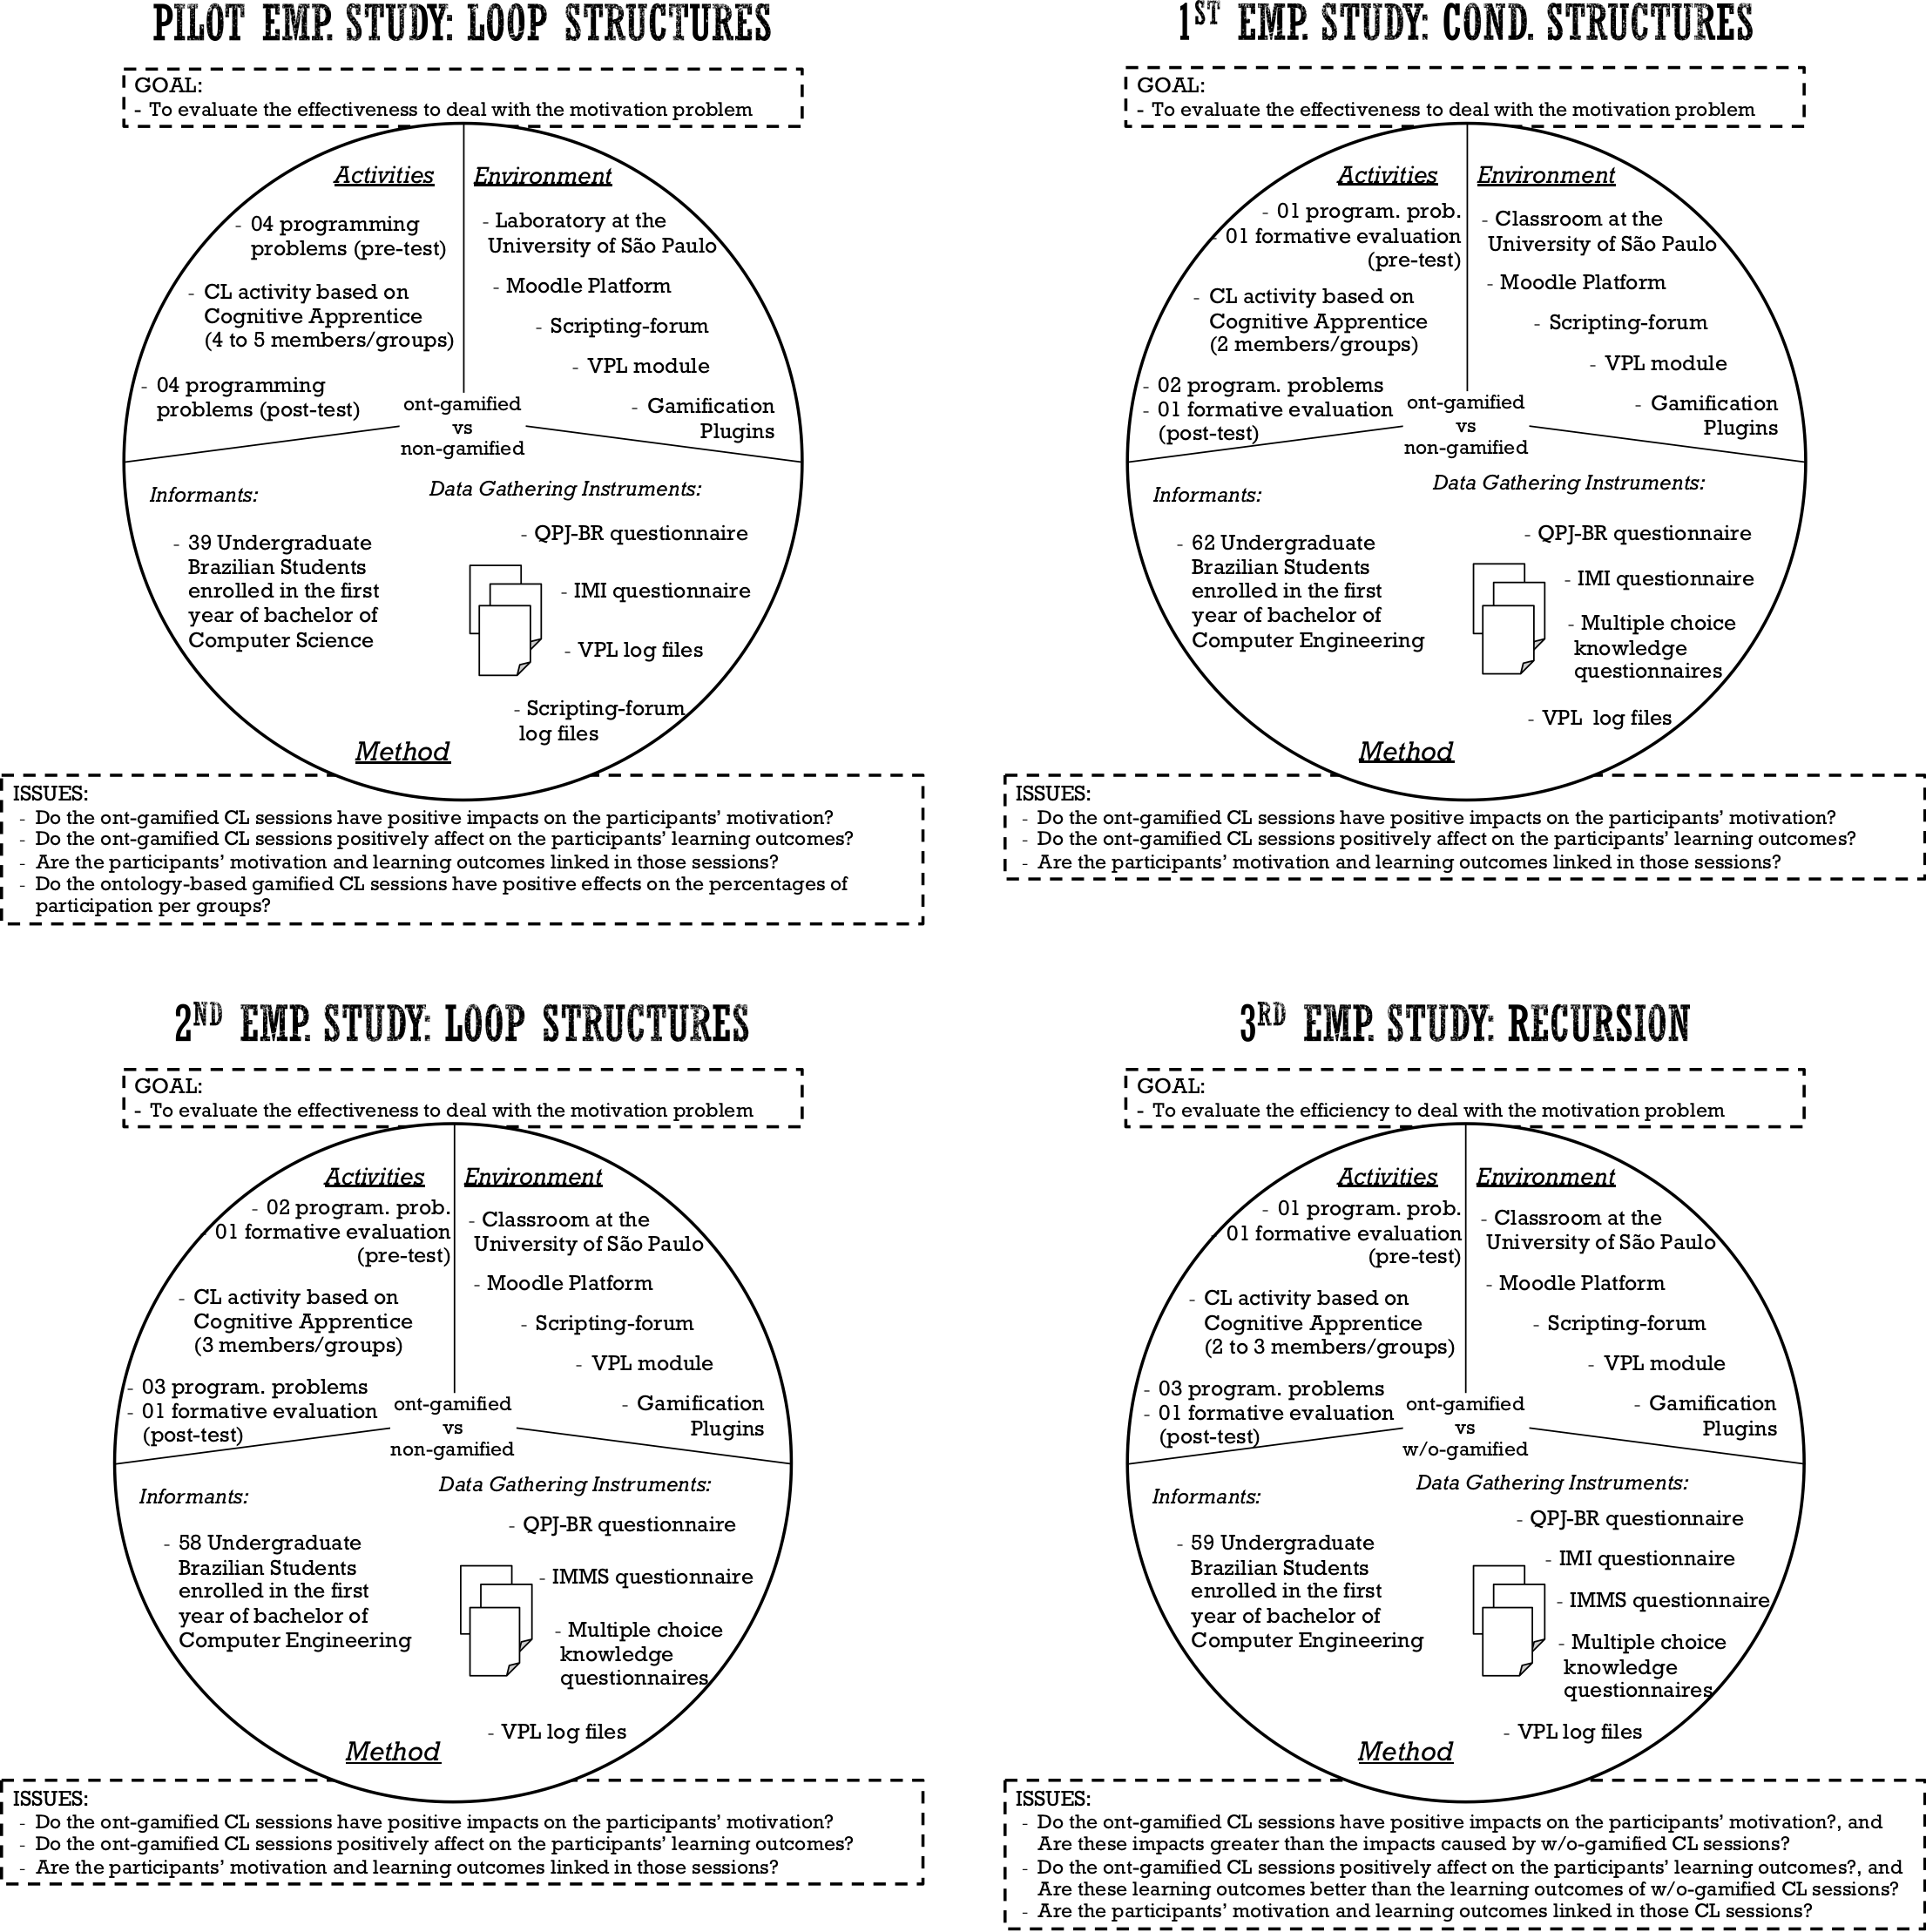
\includegraphics[width=0.95\textwidth]{images/graphical-empirical-studies.png}
 \fautor
\end{figure}

The graphical representation for each empirical studies shown in \autoref{fig:graphical-empirical-studies} is an adaptation of the Evaluand-oriented Responsive Evaluation Model (CSCL-EREM) diagram \cite{Jorrin-AbellanStakeMartinez-Mone2009}. This diagram, in the original version, is an artifact that summarizes the characteristics that should be taken into account by researchers to conduct a CSCL evaluation. The diagram employed here is a simplified version of CSCL-EREM diagram that shows only the relevant aspects of evaluating the \emph{ontological engineering approach to gamify CL scenarios} by means of empirical studies. The context of empirical studies are described at the left- and right-upper sides of diagrams, where: the right-upper side indicates the environments in which the experiment is executed, and the left-upper side 

\subsection{Planning}

\subsubsection{Design}

\subsubsection{Analysis Procedure}


\subsubsection{Evaluation of validity}




, and similitudes and differences among these studies are summarized in \autoref{tab:summary-empirical-studies}


, and the right-upper side indicates the environment in which the empirical study is executed


In the diagrams, t

in which the learning environment where the  is .


The lower side of each circle constitutes 

 part indicates the context in which 

, so that the original version consists in the representation of relevant aspects of a Cevaluation  three facets of he

within the three facets of the model, 

% Please add the following required packages to your document preamble:
% \usepackage{longtable}
% Note: It may be necessary to compile the document several times to get a multi-page table to line up properly
\begin{longtable}[c]{lllll}
\caption{Summary of the empirical studies involved in the evaluation of the ontological engineering approach}
\label{tab:summary-empirical-studies}\\
                                                                          & Pilot study                                                                                                                                                                                                        & First Study                                                                                                                                                                       & Second Study                                                                                                                                                                            & Third Study                                                                                                                                                                                                                                                        \\
\endfirsthead
%
\multicolumn{5}{c}%
{{\bfseries Table \thetable\ continued from previous page}} \\
                                                                          & Pilot study                                                                                                                                                                                                        & First Study                                                                                                                                                                       & Second Study                                                                                                                                                                            & Third Study                                                                                                                                                                                                                                                        \\
\endhead
%
Scope                                                                     &                                                                                                                                                                                                                    &                                                                                                                                                                                   &                                                                                                                                                                                         &                                                                                                                                                                                                                                                                    \\
- Object of study                                                         & \multicolumn{4}{l}{Effects of ontology-based gamified CL sessions on the students' motivation and learning outcomes}                                                                                                                                                                                                                                                                                                                                                                                                                                                                                                                                                                                                                                                                                                                                                  \\
- Purpose                                                                 & \multicolumn{4}{l}{To validate the ontology engineering approach to gamify CL scenarios}                                                                                                                                                                                                                                                                                                                                                                                                                                                                                                                                                                                                                                                                                                                                                                              \\
- Quality focus                                                           & \multicolumn{3}{l}{Effectiveness to deal with the motivation problem caused by the scripted collaboration}                                                                                                                                                                                                                                                                                                                                                                                                                                                                                       & Efficiency to deal with the motivation problem caused by the scripted collaboration                                                                                                                                                                                \\
- Perspective                                                             & \multicolumn{4}{l}{Instructional designers and practitioners who would like to know the benefits of the ontology-based CL sessions}                                                                                                                                                                                                                                                                                                                                                                                                                                                                                                                                                                                                                                                                                                                                   \\
Context                                                                   & \multicolumn{4}{l}{\begin{tabular}[c]{@{}l@{}}CL activities in which the collaboration among participants is orchestrated and structured by CSCL scripts\\ - 04 specifics real situations in the course of Introduction to Computer Science at the University of São Paulo\end{tabular}}                                                                                                                                                                                                                                                                                                                                                                                                                                                                                                                                                                              \\
- Content-domain:                                                         & Loop structures                                                                                                                                                                                                    & Conditional structures                                                                                                                                                            & Loop structures                                                                                                                                                                         & Recursion                                                                                                                                                                                                                                                          \\
- Members per group:                                                      & 4 and 5 students                                                                                                                                                                                                   & 2 students                                                                                                                                                                        & 2 and 3 students                                                                                                                                                                        & 3 students                                                                                                                                                                                                                                                         \\
- Duration:                                                               & 1 week                                                                                                                                                                                                             & 1 week                                                                                                                                                                            & 1 week                                                                                                                                                                                  & 2 week                                                                                                                                                                                                                                                             \\
Hypothesis formulation:                                                   & \begin{tabular}[c]{@{}l@{}}- Hnull: There is not significant difference\\ - Hnull: There is not significant difference in the learning outcomes\\ - Hnull: Percentage of dropout of the CL activities\end{tabular} & \begin{tabular}[c]{@{}l@{}}- Hnull: There is not significant difference intrinsic motivation\\ - Hnull: There is not significant difference in the learning outcomes\end{tabular} & \begin{tabular}[c]{@{}l@{}}- Hnull: There is not significant difference in the level of motivation\\ - Hnull: There is not significant difference in the learning outcomes\end{tabular} & \begin{tabular}[c]{@{}l@{}}- Hnull: There is not significant difference in the intrinsic motivation\\ - Hnull: There is not significant difference in the level of motivation\\ - Hnull: There is not significant difference in the learning outcomes\end{tabular} \\
Variables:                                                                & \begin{tabular}[c]{@{}l@{}}- Intrinsic Motivation (Enjoyment/)\\ - Gain Score\\ \\ -\end{tabular}                                                                                                                  & \begin{tabular}[c]{@{}l@{}}- Intrinsic Motivation (Enjoyment/)\\ - Gain Score\end{tabular}                                                                                        &                                                                                                                                                                                         &                                                                                                                                                                                                                                                                    \\
\begin{tabular}[c]{@{}l@{}}Subjects:\\ (convenient sampling)\end{tabular} & \begin{tabular}[c]{@{}l@{}}Undergraduate Computer Science Students\\ Signed Up in the first bacheler degree\end{tabular}                                                                                           & \multicolumn{3}{l}{Undergraduate Engineering Computer Students}                                                                                                                                                                                                                                                                                                                                                                                                                                                                                                                                                                                  \\
Experiment Design:                                                        &                                                                                                                                                                                                                    &                                                                                                                                                                                   &                                                                                                                                                                                         &                                                                                                                                                                                                                                                                    \\
Instrumentation:                                                          &                                                                                                                                                                                                                    &                                                                                                                                                                                   &                                                                                                                                                                                         &                                                                                                                                                                                                                                                                   
\end{longtable}


The mathematical analysis methods and procedure used in the data analysis are detailed in \autoref{sec:evaluation-analysis-procedure} .

\subsection{Design}

\subsection{Subjects}

\subsection{Objects}

\subsection{Instrumentation}

\subsection{Data Collection Procedure}

In order to find out whether the \emph{ont-gamified CL sessions} affects the students' motivation 


\subsection{Data Analysis Procedure}
\label{sec:evaluation-analysis-procedure}

Prior to perform any statistical analysis related to the motivation of participants in non-gamified, ont-gamified and w/o-gamified CL sessions, outliers refer as careless responses were removed from the self-reported data gathered by motivation surveys. Outliers identified as extreme values in these data were replaced by trimmed minimum and maximum values using the Winsorization method. The detection and treatment of careless responses and extreme values is detailed in \autoref{sec:outliers-motivation}.

To measure the students' motivation towards their participation in the CL sessions, the Rating Scale Model (RSM) was used as a psychometric instrument for analyzing the self-reported data collected by the motivation surveys. The RSM is a model based on the Item Response Theory (IRT) in which the latent trait being measured by the items is estimated in function of rating scale data \cite{George2005}. In this sense, the RMS is appropriate for the data gathered through the motivation surveys in which all the items have Likert scale response format \cite{van2013handbook}. \autoref{appendix:rsm-motivation} details the measurements of students' motivation obtained using the RSM. After having these measurements, two-way ANOVA tests has been carried out to compare the effects of different CL sessions on the students' motivation. The results on these tests has been calculated employing variations between the types of CL sessions, as well as variations between the CL roles played by the participants in these sessions.

To investigate the impact of different types of CL sessions on the learning outcomes, the gains in knowledge/skills of participants has been estimated by the Nominal Item Response Model \cite{DavidThissenLiCaiRDarrellBock2010}, and by stacking the pre-test and post-test data \cite{Wright2003}. \autoref{appendix:stacking-nominal-model} details this stacked data analysis employing the Nominal Item Response Model. After having these results, two-way ANOVA tests have carried out by comparing the learning outcomes in the different type of CL sessions and the CL roles played by the participants.

After to carried out the ANOVA tests by evaluating whether there is no significant differences on the students' motivation and learning outcomes, Pearson correlation tests have been carried out to find out whether the effects of different types of CL sessions on the students' motivation and learning outcomes are linked.

\subsection{Evaluation of validity}



After to remove careless responses and to winsorize extreme values, the validation of motivation surveys was performed using confirmatory factorial analysis (CFA) and reliability analyses for all the responses collected in each empirical study.

The validation of assumptions for the ANOVA tests and the results obtained by these tests are detailed in \autoref{appendix:anova-motivation}.

 The validation of assumptions for the ANOVA tests and the results obtained by these tests are detailed in \autoref{appendix:anova-learning-outcomes}.

This appendix also details the validation of assumptions in these measurements. 

\section{Pilot Empirical Study}
\label{sec:pilot-study}

\subsection{Execution}

\subsubsection{Hypotheis testing}

Scoping;
Selection Variables
Selection of subjects
Formulation of Hypothesis
Instrument:

%%%%%%%%%%%%%%%%%%%%%%%%%%%%%%%%%%%%%%%%%%%%%%%%

\section{Pilot Empirical Study: Data Analysis and Results}
\label{sec:data-analysis-pilot-study}

Two-way between-subjects ANOVA tests were conducted to compare the effects of ontology-based gamified CL sessions (\emph{ont-gamified}) and non-gamified CL sessions (\emph{non-gamified}) on the participants' intrinsic motivation, perceived choice, pressure/tension and effort/importance. The interaction effects between these two types of CL sessions and the CL roles, \emph{Master} and \emph{Apprentice}, are evaluated in these tests. \autoref{tab:two-way-intrinsic-motivation-pilot-study}  shows the results in which there are statistically significant difference at the $0.05$ level for the participants' intrinsic motivation and perceived choice. The effect on the intrinsic motivation for the type of CL session yielded an $F$ ratio of $F(1,26) = 4.702$, $p = 0.039$ with significant differences between non-gamified CL sessions ($mean = -0.389$ \emph{logit}) and ontology-based gamified CL sessions ($mean = 0.305$ \emph{logit}). In relation to the perceived choice, the effect for the type of CL session yielded an $F$ ratio of $F(1,26) = 6.980$, $p = 0.014$, indicating significant differences between non-gamified CL sessions ($mean = -0.316$ \emph{logit}) and ontology-based gamified CL sessions ($mean = 0.290$ \emph{logit}).

%latex.default(result_df, caption = paste("Summary of two-way ANOVA results",     in_title), size = "small", longtable = T, ctable = F, landscape = F,     rowlabel = "", where = "!htbp", file = filename, append = T)%
\setlongtables{\small
\begin{longtable}{lrrrrl}\caption{Two-way ANOVA results for the latent trait estimates of intrinsic motivation, interest/enjoyment, perceived choice, pressure/tension and effort/importance in the pilot empirical study} \tabularnewline
\hline\hline
\multicolumn{1}{l}{}&\multicolumn{1}{c}{Sum Sq}&\multicolumn{1}{c}{Df}&\multicolumn{1}{c}{F value}&\multicolumn{1}{c}{Pr(\textgreater F)}&\multicolumn{1}{c}{Sig}\tabularnewline
\hline
\endfirsthead\caption[]{\em (continued)} \tabularnewline
\hline
\multicolumn{1}{l}{}&\multicolumn{1}{c}{Sum Sq}&\multicolumn{1}{c}{Df}&\multicolumn{1}{c}{F value}&\multicolumn{1}{c}{Pr(\textgreater F)}&\multicolumn{1}{c}{Sig}\tabularnewline
\hline
\endhead
\hline
\multicolumn{6}{r}{\tiny Signif. codes:  0 \aspas{**} 0.01 \aspas{*} 0.05}
\endfoot
\label{tab:two-way-intrinsic-motivation-pilot-study}
%Intrinsic Motivation:(Intercept)&$ 0.042$&$ 1$&$0.082$&$0.777$&\tabularnewline
Intrinsic Motivation:Type&$ 2.397$&$ 1$&$4.702$&$0.039$&*\tabularnewline
%Intrinsic Motivation:CLRole&$ 0.456$&$ 1$&$0.894$&$0.353$&\tabularnewline
Intrinsic Motivation:Type:CLRole&$ 0.080$&$ 1$&$0.156$&$0.696$&\tabularnewline
Intrinsic Motivation:Residuals&$13.254$&$26$&$$&$$&\tabularnewline
%Interest/Enjoyment:(Intercept)&$ 0.483$&$ 1$&$0.208$&$0.652$&$$\tabularnewline
Interest/Enjoyment:Type&$ 8.107$&$ 1$&$3.495$&$0.073$&$$\tabularnewline
%Interest/Enjoyment:CLRole&$ 1.879$&$ 1$&$0.810$&$0.376$&$$\tabularnewline
Interest/Enjoyment:Type:CLRole&$ 0.599$&$ 1$&$0.258$&$0.616$&$$\tabularnewline
Interest/Enjoyment:Residuals&$60.314$&$26$&$$&$$&$$\tabularnewline
%Perceived Choice:(Intercept)&$ 0.103$&$ 1$&$0.195$&$0.663$&\tabularnewline
Perceived Choice:Type&$ 3.675$&$ 1$&$6.980$&$0.014$&*\tabularnewline
%Perceived Choice:CLRole&$ 0.066$&$ 1$&$0.126$&$0.725$&\tabularnewline
Perceived Choice:Type:CLRole&$ 1.050$&$ 1$&$1.994$&$0.170$&\tabularnewline
Perceived Choice:Residuals&$13.689$&$26$&$$&$$&\tabularnewline
%Pressure/Tension:(Intercept)&$ 0.017$&$ 1$&$0.036$&$0.850$&$$\tabularnewline
Pressure/Tension:Type&$ 1.125$&$ 1$&$2.472$&$0.128$&$$\tabularnewline
%Pressure/Tension:CLRole&$ 0.027$&$ 1$&$0.060$&$0.809$&$$\tabularnewline
Pressure/Tension:Type:CLRole&$ 0.012$&$ 1$&$0.026$&$0.874$&$$\tabularnewline
Pressure/Tension:Residuals&$11.838$&$26$&$$&$$&$$\tabularnewline
%Effort/Importance:(Intercept)&$ 0.010$&$ 1$&$0.019$&$0.892$&$$\tabularnewline
Effort/Importance:Type&$ 0.335$&$ 1$&$0.645$&$0.429$&$$\tabularnewline
%Effort/Importance:CLRole&$ 0.068$&$ 1$&$0.130$&$0.721$&$$\tabularnewline
Effort/Importance:Type:CLRole&$ 0.273$&$ 1$&$0.525$&$0.475$&$$\tabularnewline
Effort/Importance:Residuals&$13.516$&$26$&$$&$$&$$\tabularnewline
\hline
\end{longtable}}

Tukey post-hoc comparisons has been run to confirm the significant differences occurred between the types of CL sessions and the CL roles. \autoref{tab:post-hoc-intrinsic-motivation-pilot-study} summarizes the descriptive statistics and the results of post-hoc comparisons. According to these results, the intrinsic motivation of students who participated in ontology-based gamified CL sessions ($lsmean=0.419$ \emph{logit}, and $SE = 0.206$) is greater than the intrinsic motivation of students who participated in non-gamified CL sessions ($lsmean=-0.322$ \emph{logit}, and $SE = 0.273$) with a p-adj. value of $0.013$ and Hedges' $g=0.956$ large effect size. The interest/enjoyment of participants in ontology-based gamified CL sessions ($lsmean=0.848$ \emph{logit}, and $SE = 0.440$) is greater than the interest/enjoyment of participants in non-gamified CL sessions ($lsmean=-0.515$ \emph{logit}, and $SE = 0.582$) with a p-adj. value of $0.039$ and Hedges' $g=0.780$ medium effect size. In ontology-based gamified CL sessions, the perceived choice with $lsmean=0.382$ \emph{logit} and $SE = 0.209$ is significantly greater than the perceived choice in non-gamified CL sessions with $lsmean=-0.535$ \emph{logit} and $SE = 0.277$ at the p-adj. value of $0.031$ and Hedges' $g=0.814$ large effect size.

%latex.default(post_hoc_df, caption = paste("Descriptive statistics and Tukey post-hoc test results",     in_title), size = "small", longtable = T, ctable = F, landscape = T,     rowlabel = "", where = "!htbp", file = filename, append = T)%
\setlongtables\begin{landscape}{\scriptsize
\begin{longtable}{lrrrrrrrrrrrll}\caption{Descriptive statistics and Tukey post-hoc test results for the latent trait estimates of intrinsic motivation, interest/enjoyment, perceived choice, pressure/tension and effort/importance in the pilot empirical study} \tabularnewline
\hline\hline
\multicolumn{1}{l}{}&\multicolumn{1}{c}{N}&\multicolumn{1}{c}{mean}&\multicolumn{1}{c}{lsmean}&\multicolumn{1}{c}{SE}&\multicolumn{1}{c}{df}&\multicolumn{1}{c}{lwr.CI}&\multicolumn{1}{c}{upr.CI}&\multicolumn{1}{c}{t.ratio}&\multicolumn{1}{c}{p.value}&\multicolumn{1}{c}{p-adj.}&\multicolumn{1}{c}{g}&\multicolumn{1}{c}{sig}&\multicolumn{1}{c}{mag}\tabularnewline
\hline
\endfirsthead\caption[]{\em (continued)} \tabularnewline
\hline
\multicolumn{1}{l}{}&\multicolumn{1}{c}{N}&\multicolumn{1}{c}{mean}&\multicolumn{1}{c}{lsmean}&\multicolumn{1}{c}{SE}&\multicolumn{1}{c}{df}&\multicolumn{1}{c}{lwr.CI}&\multicolumn{1}{c}{upr.CI}&\multicolumn{1}{c}{t.ratio}&\multicolumn{1}{c}{p.value}&\multicolumn{1}{c}{p-adj.}&\multicolumn{1}{c}{g}&\multicolumn{1}{c}{sig}&\multicolumn{1}{c}{mag}\tabularnewline
\hline
\endhead
\hline
\multicolumn{14}{r}{\tiny Signif. codes:  0 \aspas{**} 0.01 \aspas{*} 0.05} 
\endfoot
\label{tab:post-hoc-intrinsic-motivation-pilot-study}
Intrinsic Motivation:non-gamified&$14$&$-0.389$&$-0.322$&$0.273$&$26$&$-0.882$&$ 0.239$&$$&$$&$$&$$&&\tabularnewline
Intrinsic Motivation:ont-gamified&$16$&$ 0.305$&$ 0.419$&$0.206$&$26$&$-0.004$&$ 0.843$&$$&$$&$$&$$&&\tabularnewline
Intrinsic Motivation:non-gamified - ont-gamified&$30$&$-0.694$&$-0.741$&$0.342$&$$&$-1.231$&$-0.157$&$-2.168$&$0.039$&$0.013$&$-0.956$&*&large\tabularnewline
Intrinsic Motivation:non-gamified.Apprentice&$12$&$-0.416$&$-0.416$&$0.206$&$26$&$-0.839$&$ 0.008$&$$&$$&$$&$$&&\tabularnewline
Intrinsic Motivation:ont-gamified.Apprentice&$12$&$ 0.190$&$ 0.190$&$0.206$&$26$&$-0.233$&$ 0.614$&$$&$$&$$&$$&&\tabularnewline
Intrinsic Motivation:non-gamified.Apprentice - ont-gamified.Apprentice&$24$&$-0.606$&$-0.606$&$0.291$&$$&$-1.406$&$ 0.194$&$-2.079$&$0.048$&$0.186$&$-0.818$&&\tabularnewline
Intrinsic Motivation:non-gamified.Master&$ 2$&$-0.228$&$-0.228$&$0.505$&$26$&$-1.266$&$ 0.810$&$$&$$&$$&$$&&\tabularnewline
Intrinsic Motivation:ont-gamified.Master&$ 4$&$ 0.649$&$ 0.649$&$0.357$&$26$&$-0.085$&$ 1.382$&$$&$$&$$&$$&&\tabularnewline
Intrinsic Motivation:non-gamified.Master - ont-gamified.Master&$ 6$&$-0.876$&$-0.876$&$0.618$&$$&$-2.573$&$ 0.820$&$-1.417$&$0.168$&$0.500$&$-0.991$&&\tabularnewline
\hline

Interest/Enjoyment:non-gamified&$14$&$-0.617$&$-0.515$&$0.582$&$26$&$-1.711$&$ 0.680$&$$&$$&$$&$$&&\tabularnewline
Interest/Enjoyment:ont-gamified&$16$&$ 0.591$&$ 0.848$&$0.440$&$26$&$-0.056$&$ 1.752$&$$&$$&$$&$$&&\tabularnewline
Interest/Enjoyment:non-gamified - ont-gamified&$30$&$-1.208$&$-1.363$&$0.729$&$$&$-2.354$&$-0.063$&$-1.869$&$0.073$&$0.039$&$-0.780$&*&medium\tabularnewline
Interest/Enjoyment:non-gamified.Apprentice&$12$&$-0.658$&$-0.658$&$0.440$&$26$&$-1.562$&$ 0.246$&$$&$$&$$&$$&&\tabularnewline
Interest/Enjoyment:ont-gamified.Apprentice&$12$&$ 0.335$&$ 0.335$&$0.440$&$26$&$-0.569$&$ 1.238$&$$&$$&$$&$$&&\tabularnewline
Interest/Enjoyment:non-gamified.Apprentice - ont-gamified.Apprentice&$24$&$-0.993$&$-0.993$&$0.622$&$$&$-2.698$&$ 0.713$&$-1.596$&$0.123$&$0.398$&$-0.612$&&\tabularnewline
Interest/Enjoyment:non-gamified.Master&$ 2$&$-0.372$&$-0.372$&$1.077$&$26$&$-2.586$&$ 1.841$&$$&$$&$$&$$&&\tabularnewline
Interest/Enjoyment:ont-gamified.Master&$ 4$&$ 1.361$&$ 1.361$&$0.762$&$26$&$-0.204$&$ 2.927$&$$&$$&$$&$$&&\tabularnewline
Interest/Enjoyment:non-gamified.Master - ont-gamified.Master&$ 6$&$-1.734$&$-1.734$&$1.319$&$$&$-5.352$&$ 1.885$&$-1.314$&$0.200$&$0.562$&$-1.100$&&\tabularnewline
\hline

Perceived Choice:non-gamified&$14$&$-0.316$&$-0.535$&$0.277$&$26$&$-1.105$&$ 0.034$&$$&$$&$$&$$&&\tabularnewline
Perceived Choice:ont-gamified&$16$&$ 0.290$&$ 0.382$&$0.209$&$26$&$-0.048$&$ 0.813$&$$&$$&$$&$$&&\tabularnewline
Perceived Choice:non-gamified - ont-gamified&$30$&$-0.607$&$-0.918$&$0.347$&$$&$-1.152$&$-0.061$&$-2.642$&$0.014$&$0.031$&$-0.814$&*&large\tabularnewline
Perceived Choice:non-gamified.Apprentice&$12$&$-0.229$&$-0.229$&$0.209$&$26$&$-0.659$&$ 0.202$&$$&$$&$$&$$&&\tabularnewline
Perceived Choice:ont-gamified.Apprentice&$12$&$ 0.199$&$ 0.199$&$0.209$&$26$&$-0.232$&$ 0.629$&$$&$$&$$&$$&&\tabularnewline
Perceived Choice:non-gamified.Apprentice - ont-gamified.Apprentice&$24$&$-0.427$&$-0.427$&$0.296$&$$&$-1.240$&$ 0.386$&$-1.442$&$0.161$&$0.486$&$-0.557$&&\tabularnewline
Perceived Choice:non-gamified.Master&$ 2$&$-0.842$&$-0.842$&$0.513$&$26$&$-1.897$&$ 0.212$&$$&$$&$$&$$&&\tabularnewline
Perceived Choice:ont-gamified.Master&$ 4$&$ 0.566$&$ 0.566$&$0.363$&$26$&$-0.180$&$ 1.312$&$$&$$&$$&$$&&\tabularnewline
Perceived Choice:non-gamified.Master - ont-gamified.Master&$ 6$&$-1.408$&$-1.408$&$0.628$&$$&$-3.132$&$ 0.316$&$-2.241$&$0.034$&$0.139$&$-1.767$&&\tabularnewline
\newpage

Pressure/Tension:non-gamified&$14$&$ 0.238$&$ 0.285$&$0.258$&$26$&$-0.245$&$0.814$&$$&$$&$$&$$&$$&$$\tabularnewline
Pressure/Tension:ont-gamified&$16$&$-0.230$&$-0.223$&$0.195$&$26$&$-0.624$&$0.177$&$$&$$&$$&$$&$$&$$\tabularnewline
Pressure/Tension:non-gamified - ont-gamified&$30$&$ 0.468$&$ 0.508$&$0.323$&$$&$-0.040$&$0.976$&$1.572$&$0.128$&$0.069$&$0.699$&$$&$$\tabularnewline
Pressure/Tension:non-gamified.Apprentice&$12$&$ 0.219$&$ 0.219$&$0.195$&$26$&$-0.181$&$0.620$&$$&$$&$$&$$&$$&$$\tabularnewline
Pressure/Tension:ont-gamified.Apprentice&$12$&$-0.237$&$-0.237$&$0.195$&$26$&$-0.637$&$0.164$&$$&$$&$$&$$&$$&$$\tabularnewline
Pressure/Tension:non-gamified.Apprentice - ont-gamified.Apprentice&$24$&$ 0.456$&$ 0.456$&$0.275$&$$&$-0.300$&$1.212$&$1.656$&$0.110$&$0.366$&$0.624$&$$&$$\tabularnewline
Pressure/Tension:non-gamified.Master&$ 2$&$ 0.350$&$ 0.350$&$0.477$&$26$&$-0.631$&$1.331$&$$&$$&$$&$$&$$&$$\tabularnewline
Pressure/Tension:ont-gamified.Master&$ 4$&$-0.210$&$-0.210$&$0.337$&$26$&$-0.903$&$0.484$&$$&$$&$$&$$&$$&$$\tabularnewline
Pressure/Tension:non-gamified.Master - ont-gamified.Master&$ 6$&$ 0.560$&$ 0.560$&$0.584$&$$&$-1.044$&$2.163$&$0.958$&$0.347$&$0.774$&$0.950$&$$&$$\tabularnewline
\hline

Effort/Importance:non-gamified&$14$&$ 0.028$&$ 0.162$&$0.275$&$26$&$-0.404$&$0.728$&$$&$$&$$&$$&$$&$$\tabularnewline
Effort/Importance:ont-gamified&$16$&$-0.084$&$-0.115$&$0.208$&$26$&$-0.543$&$0.313$&$$&$$&$$&$$&$$&$$\tabularnewline
Effort/Importance:non-gamified - ont-gamified&$30$&$ 0.112$&$ 0.277$&$0.345$&$$&$-0.430$&$0.654$&$0.803$&$0.429$&$0.674$&$0.155$&$$&$$\tabularnewline
Effort/Importance:non-gamified.Apprentice&$12$&$-0.025$&$-0.025$&$0.208$&$26$&$-0.453$&$0.403$&$$&$$&$$&$$&$$&$$\tabularnewline
Effort/Importance:ont-gamified.Apprentice&$12$&$-0.052$&$-0.052$&$0.208$&$26$&$-0.480$&$0.376$&$$&$$&$$&$$&$$&$$\tabularnewline
Effort/Importance:non-gamified.Apprentice - ont-gamified.Apprentice&$24$&$ 0.027$&$ 0.027$&$0.294$&$$&$-0.780$&$0.835$&$0.092$&$0.927$&$1.000$&$0.037$&$$&$$\tabularnewline
Effort/Importance:non-gamified.Master&$ 2$&$ 0.349$&$ 0.349$&$0.510$&$26$&$-0.699$&$1.397$&$$&$$&$$&$$&$$&$$\tabularnewline
Effort/Importance:ont-gamified.Master&$ 4$&$-0.178$&$-0.178$&$0.361$&$26$&$-0.919$&$0.563$&$$&$$&$$&$$&$$&$$\tabularnewline
Effort/Importance:non-gamified.Master - ont-gamified.Master&$ 6$&$ 0.527$&$ 0.527$&$0.624$&$$&$-1.186$&$2.240$&$0.844$&$0.406$&$0.833$&$0.545$&$$&$$\tabularnewline
\hline
\end{longtable}}\end{landscape}


%%%%%%%%%%%%%%%%%%%%%%%%%%%%%%%%%%%%%%%%%%%%%%%%
\section{First Empirical Study: Data Analysis and Results}
\label{sec:first-study}

\autoref{tab:two-way-intrinsic-motivation-first-study} shows the results of two-way between-subjects ANOVA tests conducted to compare the effects of ontology-based gamified CL sessions (\emph{ont-gamified}) and non-gamified CL sessions (\emph{non-gamified}) on the participants' intrinsic motivation, interest/enjoyment, perceived choice, pressure/tension and effort/importance. According to these results, there are statistically significant difference at the $0.05$ level for the participants' intrinsic motivation, interest/enjoyment, pressure/tension and effort/importance. On the intrinsic motivation, the effect for the type of CL session yielded a $F$ ratio of $F(1,56) = 8.103$ and $p = 0.006$ indicating significant differences between non-gamified CL sessions ($mean = -0.329$ \emph{logit}) and ontology-based gamified CL sessions ($mean = 0.129$ \emph{logit}). The effect on the perceived choice for the type of CL session yielded a $F$ ratio of $F(1,56) = 7.885$ and $p = 0.007$ indicating significant differences between non-gamified CL sessions ($mean = -0.340$ \emph{logit}) and ontology-based gamified CL sessions ($mean = 0.310$ \emph{logit}). On the pressure/tension, the effect for the type of CL session and CL role yielded a $F$ ratio of $F(1,56) = 6.151$ and $p = 0.016$ indicating significant differences between apprentices of non-gamified CL sessions ($mean = 0.817$) and apprentices of ontology-based gamified CL sessions ($mean = -0.237$). The effect on the effort/importance for the type of CL session yielded a $F$ ratio of $F(1,56) = 4.303$ and $p = 0.043$ indicating significant differences between non-gamified CL sessions ($mean = -0.311$ \emph{logit}) and ontology-based gamified CL sessions ($mean = 0.218$ \emph{logit}).


%latex.default(result_df, caption = paste("Summary of two-way ANOVA results",     in_title), size = "small", longtable = T, ctable = F, landscape = F,     rowlabel = "", where = "!htbp", file = filename, append = T)%
\setlongtables{\small
\begin{longtable}{lrrrrl}\caption{Two-way ANOVA for the latent trait estimates of intrinsic motivation, interest/enjoyment, perceived choice, pressure/tension and effort/importance in the first empirical study} \tabularnewline
\hline\hline
\multicolumn{1}{l}{}&\multicolumn{1}{c}{Sum Sq}&\multicolumn{1}{c}{Df}&\multicolumn{1}{c}{F value}&\multicolumn{1}{c}{Pr(\textgreater F)}&\multicolumn{1}{c}{Sig}\tabularnewline
\hline
\endfirsthead\caption[]{\em (continued)} \tabularnewline
\hline
\multicolumn{1}{l}{}&\multicolumn{1}{c}{Sum Sq}&\multicolumn{1}{c}{Df}&\multicolumn{1}{c}{F value}&\multicolumn{1}{c}{Pr(\textgreater F)}&\multicolumn{1}{c}{Sig}\tabularnewline
\hline
\endhead
\hline
\multicolumn{6}{r}{\tiny Signif. codes:  0 \aspas{**} 0.01 \aspas{*} 0.05}
\endfoot
\label{tab:two-way-intrinsic-motivation-first-study}
%Intrinsic Motivation:(Intercept)&$ 0.579$&$ 1$&$1.520$&$0.223$&\tabularnewline
Intrinsic Motivation:Type&$ 3.087$&$ 1$&$8.103$&$0.006$&**\tabularnewline
%Intrinsic Motivation:CLRole&$ 0.064$&$ 1$&$0.168$&$0.683$&\tabularnewline
Intrinsic Motivation:Type:CLRole&$ 0.020$&$ 1$&$0.053$&$0.819$&\tabularnewline
Intrinsic Motivation:Residuals&$21.333$&$56$&$$&$$&\tabularnewline
%Interest/Enjoyment:(Intercept)&$ 0.421$&$ 1$&$0.419$&$0.520$&$$\tabularnewline
Interest/Enjoyment:Type&$ 0.946$&$ 1$&$0.942$&$0.336$&$$\tabularnewline
%Interest/Enjoyment:CLRole&$ 0.268$&$ 1$&$0.267$&$0.607$&$$\tabularnewline
Interest/Enjoyment:Type:CLRole&$ 2.003$&$ 1$&$1.993$&$0.164$&$$\tabularnewline
Interest/Enjoyment:Residuals&$52.258$&$52$&$$&$$&$$\tabularnewline
%Perceived Choice:(Intercept)&$ 0.016$&$ 1$&$0.020$&$0.889$&\tabularnewline
Perceived Choice:Type&$ 6.371$&$ 1$&$7.885$&$0.007$&**\tabularnewline
%Perceived Choice:CLRole&$ 0.229$&$ 1$&$0.283$&$0.597$&\tabularnewline
Perceived Choice:Type:CLRole&$ 0.050$&$ 1$&$0.061$&$0.805$&\tabularnewline
Perceived Choice:Residuals&$45.244$&$56$&$$&$$&\tabularnewline
%Pressure/Tension:(Intercept)&$ 5.506$&$ 1$&$5.333$&$0.025$&\tabularnewline
Pressure/Tension:Type&$ 2.428$&$ 1$&$2.352$&$0.131$&\tabularnewline
%Pressure/Tension:CLRole&$ 0.011$&$ 1$&$0.011$&$0.918$&\tabularnewline
Pressure/Tension:Type:CLRole&$ 6.351$&$ 1$&$6.151$&$0.016$&*\tabularnewline
Pressure/Tension:Residuals&$57.815$&$56$&$$&$$&\tabularnewline
%Effort/Importance:(Intercept)&$ 0.078$&$ 1$&$0.086$&$0.770$&\tabularnewline
Effort/Importance:Type&$ 3.861$&$ 1$&$4.303$&$0.043$&*\tabularnewline
%Effort/Importance:CLRole&$ 2.374$&$ 1$&$2.646$&$0.109$&\tabularnewline
Effort/Importance:Type:CLRole&$ 0.799$&$ 1$&$0.891$&$0.349$&\tabularnewline
Effort/Importance:Residuals&$50.244$&$56$&$$&$$&\tabularnewline
\hline
\end{longtable}}

The results of Tukey post-hoc comparisons to confirm the significant differences in the participants' motivation occurred between the types of CL sessions and the CL roles in the first empirical study are shown in \autoref{tab:post-hoc-intrinsic-motivation-first-study}. According to these results, the intrinsic motivation of participants in ontology-based gamified CL sessions ($lsmean=0.129$ \emph{logit}, and $SE = 0.113$) is greater than the intrinsic motivation of participants in non-gamified CL sessions ($lsmean=-0.325$ \emph{logit}, and $SE = 0.113$) with a p-adj. value of $0.006$ and Hedges' $g=0.743$ meium effect size. The perceived choice of participants in ontology-based gamified CL sessions ($lsmean=0.310$ \emph{logit}, and $SE = 0.164$) is greater than the perceived choice of participants in non-gamified CL sessions ($lsmean=-0.343$ \emph{logit}, and $SE = 0.164$) with a p-adj. value of $0.007$ and Hedges' $g=0.724$ medium effect size. The pressure/tension of apprentices in ontology-based gamified CL sessions ($lsmean=-0.237$ \emph{logit}, and $SE = 0.262$) is less than apprentices in non-gamified CL sessions ($lsmean=0.817$ \emph{logit}, and $SE = 0.272$) with a p-adj. value of $0.035$ and Hedges' $g=0.964$ large effect size. The participants' effort/importance in ontology-based CL sessions ($lsmean=0.218$ \emph{logit}, and $SE = 0.173$) is greater than the participants' effort/importance in non-gamified CL sessions ($lsmean=-0.290$ \emph{logit}, and $SE = 0.173$) with a p-adj. value of $0.035$ and Hedges' $g=0.544$ medium effect size.

%latex.default(post_hoc_df, caption = paste("Descriptive statistics and Tukey post-hoc test results",     in_title), size = "small", longtable = T, ctable = F, landscape = T,     rowlabel = "", where = "!htbp", file = filename, append = T)%
\setlongtables\begin{landscape}{\scriptsize
\begin{longtable}{lrrrrrrrrrrrll}\caption{Descriptive statistics and Tukey post-hoc test results for the latent trait estimates of intrinsic motivation, interest/enjoyment, perceived choice, pressure/tension and effort/importance in the first empirical study} \tabularnewline
\hline\hline
\multicolumn{1}{l}{}&\multicolumn{1}{c}{N}&\multicolumn{1}{c}{mean}&\multicolumn{1}{c}{lsmean}&\multicolumn{1}{c}{SE}&\multicolumn{1}{c}{df}&\multicolumn{1}{c}{lwr.CI}&\multicolumn{1}{c}{upr.CI}&\multicolumn{1}{c}{t.ratio}&\multicolumn{1}{c}{p.value}&\multicolumn{1}{c}{p-adj.}&\multicolumn{1}{c}{g}&\multicolumn{1}{c}{sig}&\multicolumn{1}{c}{mag}\tabularnewline
\hline
\endfirsthead\caption[]{\em (continued)} \tabularnewline
\hline
\multicolumn{1}{l}{}&\multicolumn{1}{c}{N}&\multicolumn{1}{c}{mean}&\multicolumn{1}{c}{lsmean}&\multicolumn{1}{c}{SE}&\multicolumn{1}{c}{df}&\multicolumn{1}{c}{lwr.CI}&\multicolumn{1}{c}{upr.CI}&\multicolumn{1}{c}{t.ratio}&\multicolumn{1}{c}{p.value}&\multicolumn{1}{c}{p-adj.}&\multicolumn{1}{c}{g}&\multicolumn{1}{c}{sig}&\multicolumn{1}{c}{mag}\tabularnewline
\hline
\endhead
\hline
\multicolumn{14}{r}{\tiny Signif. codes:  0 \aspas{**} 0.01 \aspas{*} 0.05}
\endfoot
\label{tab:post-hoc-intrinsic-motivation-first-study}
Intrinsic Motivation:non-gamified&$30$&$-0.329$&$-0.325$&$0.113$&$56$&$-0.552$&$-0.099$&$$&$$&$$&$$&&\tabularnewline
Intrinsic Motivation:ont-gamified&$30$&$ 0.129$&$ 0.129$&$0.113$&$56$&$-0.097$&$ 0.354$&$$&$$&$$&$$&&\tabularnewline
Intrinsic Motivation:non-gamified - ont-gamified&$60$&$-0.458$&$-0.454$&$0.160$&$$&$-0.777$&$-0.138$&$-2.847$&$0.006$&$0.006$&$-0.743$&**&medium\tabularnewline
Intrinsic Motivation:non-gamified.Apprentice&$14$&$-0.274$&$-0.274$&$0.165$&$56$&$-0.605$&$ 0.056$&$$&$$&$$&$$&&\tabularnewline
Intrinsic Motivation:ont-gamified.Apprentice&$15$&$ 0.143$&$ 0.143$&$0.159$&$56$&$-0.176$&$ 0.462$&$$&$$&$$&$$&&\tabularnewline
Intrinsic Motivation:non-gamified.Apprentice - ont-gamified.Apprentice&$29$&$-0.418$&$-0.418$&$0.229$&$$&$-1.025$&$ 0.190$&$-1.820$&$0.074$&$0.275$&$-0.583$&&\tabularnewline
Intrinsic Motivation:non-gamified.Master&$16$&$-0.376$&$-0.376$&$0.154$&$56$&$-0.686$&$-0.067$&$$&$$&$$&$$&&\tabularnewline
Intrinsic Motivation:ont-gamified.Master&$15$&$ 0.114$&$ 0.114$&$0.159$&$56$&$-0.205$&$ 0.434$&$$&$$&$$&$$&&\tabularnewline
Intrinsic Motivation:non-gamified.Master - ont-gamified.Master&$31$&$-0.491$&$-0.491$&$0.222$&$$&$-1.078$&$ 0.097$&$-2.212$&$0.031$&$0.132$&$-0.896$&&\tabularnewline
\hline

Interest/Enjoyment:non-gamified&$28$&$-0.217$&$-0.217$&$0.189$&$52$&$-0.597$&$0.163$&$$&$$&$$&$$&$$&$$\tabularnewline
Interest/Enjoyment:ont-gamified&$28$&$ 0.062$&$ 0.043$&$0.190$&$52$&$-0.338$&$0.424$&$$&$$&$$&$$&$$&$$\tabularnewline
Interest/Enjoyment:non-gamified - ont-gamified&$56$&$-0.279$&$-0.260$&$0.268$&$$&$-0.816$&$0.259$&$-0.970$&$0.336$&$0.303$&$-0.274$&$$&$$\tabularnewline
Interest/Enjoyment:non-gamified.Apprentice&$14$&$-0.097$&$-0.097$&$0.268$&$52$&$-0.635$&$0.441$&$$&$$&$$&$$&$$&$$\tabularnewline
Interest/Enjoyment:ont-gamified.Apprentice&$13$&$-0.215$&$-0.215$&$0.278$&$52$&$-0.773$&$0.343$&$$&$$&$$&$$&$$&$$\tabularnewline
Interest/Enjoyment:non-gamified.Apprentice - ont-gamified.Apprentice&$27$&$ 0.118$&$ 0.118$&$0.386$&$$&$-0.906$&$1.143$&$ 0.307$&$0.760$&$0.990$&$ 0.106$&$$&$$\tabularnewline
Interest/Enjoyment:non-gamified.Master&$14$&$-0.337$&$-0.337$&$0.268$&$52$&$-0.875$&$0.201$&$$&$$&$$&$$&$$&$$\tabularnewline
Interest/Enjoyment:ont-gamified.Master&$15$&$ 0.302$&$ 0.302$&$0.259$&$52$&$-0.217$&$0.821$&$$&$$&$$&$$&$$&$$\tabularnewline
Interest/Enjoyment:non-gamified.Master - ont-gamified.Master&$29$&$-0.639$&$-0.639$&$0.373$&$$&$-1.628$&$0.350$&$-1.715$&$0.092$&$0.326$&$-0.678$&$$&$$\tabularnewline
\hline

Perceived Choice:non-gamified&$30$&$-0.340$&$-0.343$&$0.164$&$56$&$-0.672$&$-0.013$&$$&$$&$$&$$&&\tabularnewline
Perceived Choice:ont-gamified&$30$&$ 0.310$&$ 0.310$&$0.164$&$56$&$-0.019$&$ 0.639$&$$&$$&$$&$$&&\tabularnewline
Perceived Choice:non-gamified - ont-gamified&$60$&$-0.650$&$-0.652$&$0.232$&$$&$-1.115$&$-0.185$&$-2.808$&$0.007$&$0.007$&$-0.724$&**&medium\tabularnewline
Perceived Choice:non-gamified.Apprentice&$14$&$-0.376$&$-0.376$&$0.240$&$56$&$-0.857$&$ 0.106$&$$&$$&$$&$$&&\tabularnewline
Perceived Choice:ont-gamified.Apprentice&$15$&$ 0.219$&$ 0.219$&$0.232$&$56$&$-0.246$&$ 0.684$&$$&$$&$$&$$&&\tabularnewline
Perceived Choice:non-gamified.Apprentice - ont-gamified.Apprentice&$29$&$-0.595$&$-0.595$&$0.334$&$$&$-1.479$&$ 0.290$&$-1.781$&$0.080$&$0.293$&$-0.617$&&\tabularnewline
Perceived Choice:non-gamified.Master&$16$&$-0.310$&$-0.310$&$0.225$&$56$&$-0.760$&$ 0.141$&$$&$$&$$&$$&&\tabularnewline
Perceived Choice:ont-gamified.Master&$15$&$ 0.401$&$ 0.401$&$0.232$&$56$&$-0.064$&$ 0.865$&$$&$$&$$&$$&&\tabularnewline
Perceived Choice:non-gamified.Master - ont-gamified.Master&$31$&$-0.710$&$-0.710$&$0.323$&$$&$-1.565$&$ 0.145$&$-2.198$&$0.032$&$0.136$&$-0.802$&&\tabularnewline
\newpage

Pressure/Tension:non-gamified&$30$&$ 0.484$&$ 0.505$&$0.186$&$56$&$ 0.132$&$0.877$&$$&$$&$$&$$&&\tabularnewline
Pressure/Tension:ont-gamified&$30$&$ 0.102$&$ 0.102$&$0.186$&$56$&$-0.270$&$0.473$&$$&$$&$$&$$&&\tabularnewline
Pressure/Tension:non-gamified - ont-gamified&$60$&$ 0.382$&$ 0.403$&$0.263$&$$&$-0.144$&$0.908$&$ 1.534$&$0.131$&$0.151$&$ 0.358$&&\tabularnewline
Pressure/Tension:non-gamified.Apprentice&$14$&$ 0.817$&$ 0.817$&$0.272$&$56$&$ 0.273$&$1.361$&$$&$$&$$&$$&&\tabularnewline
Pressure/Tension:ont-gamified.Apprentice&$15$&$-0.237$&$-0.237$&$0.262$&$56$&$-0.763$&$0.288$&$$&$$&$$&$$&&\tabularnewline
Pressure/Tension:non-gamified.Apprentice - ont-gamified.Apprentice&$29$&$ 1.054$&$ 1.054$&$0.378$&$$&$ 0.054$&$2.054$&$ 2.792$&$0.007$&$0.035$&$ 0.964$&*&large\tabularnewline
Pressure/Tension:non-gamified.Master&$16$&$ 0.193$&$ 0.193$&$0.254$&$56$&$-0.316$&$0.701$&$$&$$&$$&$$&&\tabularnewline
Pressure/Tension:ont-gamified.Master&$15$&$ 0.441$&$ 0.441$&$0.262$&$56$&$-0.084$&$0.967$&$$&$$&$$&$$&&\tabularnewline
Pressure/Tension:non-gamified.Master - ont-gamified.Master&$31$&$-0.249$&$-0.249$&$0.365$&$$&$-1.216$&$0.718$&$-0.681$&$0.499$&$0.904$&$-0.249$&&\tabularnewline
\hline

Effort/Importance:non-gamified&$30$&$-0.311$&$-0.290$&$0.173$&$56$&$-0.637$&$ 0.057$&$$&$$&$$&$$&&\tabularnewline
Effort/Importance:ont-gamified&$30$&$ 0.218$&$ 0.218$&$0.173$&$56$&$-0.128$&$ 0.564$&$$&$$&$$&$$&&\tabularnewline
Effort/Importance:non-gamified - ont-gamified&$60$&$-0.529$&$-0.508$&$0.245$&$$&$-1.019$&$-0.039$&$-2.074$&$0.043$&$0.035$&$-0.544$&*&medium\tabularnewline
Effort/Importance:non-gamified.Apprentice&$14$&$ 0.025$&$ 0.025$&$0.253$&$56$&$-0.482$&$ 0.532$&$$&$$&$$&$$&&\tabularnewline
Effort/Importance:ont-gamified.Apprentice&$15$&$ 0.302$&$ 0.302$&$0.245$&$56$&$-0.188$&$ 0.792$&$$&$$&$$&$$&&\tabularnewline
Effort/Importance:non-gamified.Apprentice - ont-gamified.Apprentice&$29$&$-0.277$&$-0.277$&$0.352$&$$&$-1.209$&$ 0.655$&$-0.786$&$0.435$&$0.860$&$-0.260$&&\tabularnewline
Effort/Importance:non-gamified.Master&$16$&$-0.605$&$-0.605$&$0.237$&$56$&$-1.079$&$-0.130$&$$&$$&$$&$$&&\tabularnewline
Effort/Importance:ont-gamified.Master&$15$&$ 0.134$&$ 0.134$&$0.245$&$56$&$-0.356$&$ 0.624$&$$&$$&$$&$$&&\tabularnewline
Effort/Importance:non-gamified.Master - ont-gamified.Master&$31$&$-0.739$&$-0.739$&$0.340$&$$&$-1.640$&$ 0.162$&$-2.171$&$0.034$&$0.144$&$-0.839$&&\tabularnewline
\hline
\end{longtable}}\end{landscape}




%%%%%%%%%%%%%%%%%%%%%%%%%%%%%%%%%%%%%%%%%%%%%%%%
\section{Data Analysis: Second Empirical Study}
\label{sec:second-study}


\autoref{tab:two-way-intrinsic-motivation-second-study} shows the results of two-way between-subjects ANOVA tests conducted to compare the effects of ontology-based gamified CL sessions (\emph{ont-gamified}) and non-gamified CL sessions (\emph{non-gamified}) on the participants' level of motivation, attention, relevance and satistifaction. According to these results, there were no statistically significant differences at the $0.05$ level. 

%latex.default(result_df, caption = paste("Summary of two-way ANOVA results",     in_title), size = "small", longtable = T, ctable = F, landscape = F,     rowlabel = "", where = "!htbp", file = filename, append = T)%
\setlongtables{\small
\begin{longtable}{lrrrrr}\caption{Two-way ANOVA results  for the latent trait estimates of level of motivation, attention, relevance and satisfaction in the second empirical study} \tabularnewline
\hline\hline
\multicolumn{1}{l}{}&\multicolumn{1}{c}{Sum Sq}&\multicolumn{1}{c}{Df}&\multicolumn{1}{c}{F value}&\multicolumn{1}{c}{Pr(\textgreater F)}&\multicolumn{1}{c}{Sig}\tabularnewline
\hline
\endfirsthead\caption[]{\em (continued)} \tabularnewline
\hline
\multicolumn{1}{l}{}&\multicolumn{1}{c}{Sum Sq}&\multicolumn{1}{c}{Df}&\multicolumn{1}{c}{F value}&\multicolumn{1}{c}{Pr(\textgreater F)}&\multicolumn{1}{c}{Sig}\tabularnewline
\hline
\endhead
\hline
\multicolumn{6}{r}{\tiny Signif. codes:  0 \aspas{**} 0.01 \aspas{*} 0.05}
\endfoot
\label{tab:two-way-intrinsic-motivation-second-study}
%Level of Motivation:(Intercept)&$ 0.003$&$ 1$&$0.005$&$0.947$&$$\tabularnewline
Level of Motivation:Type&$ 0.261$&$ 1$&$0.345$&$0.559$&$$\tabularnewline
%Level of Motivation:CLRole&$ 0.011$&$ 1$&$0.015$&$0.903$&$$\tabularnewline
Level of Motivation:Type:CLRole&$ 0.770$&$ 1$&$1.022$&$0.317$&$$\tabularnewline
Level of Motivation:Residuals&$40.727$&$54$&$$&$$&$$\tabularnewline
%Attention:;(Intercept)&$ 0.028$&$ 1$&$0.018$&$0.893$&$$\tabularnewline
Attention:Type&$ 1.605$&$ 1$&$1.031$&$0.314$&$$\tabularnewline
%Attention:CLRole&$ 0.006$&$ 1$&$0.004$&$0.951$&$$\tabularnewline
Attention:Type:CLRole&$ 2.002$&$ 1$&$1.286$&$0.262$&$$\tabularnewline
Attention:Residuals&$84.055$&$54$&$$&$$&$$\tabularnewline
%Relevance:(Intercept)&$ 0.002$&$ 1$&$0.005$&$0.946$&$$\tabularnewline
Relevance:Type&$ 0.057$&$ 1$&$0.116$&$0.735$&$$\tabularnewline
%Relevance:CLRole&$ 0.153$&$ 1$&$0.310$&$0.580$&$$\tabularnewline
Relevance:Type:CLRole&$ 0.016$&$ 1$&$0.033$&$0.856$&$$\tabularnewline
Relevance:Residuals&$26.662$&$54$&$$&$$&$$\tabularnewline
%Satisfaction:(Intercept)&$ 0.002$&$ 1$&$0.001$&$0.969$&$$\tabularnewline
Satisfaction:Type&$ 0.084$&$ 1$&$0.056$&$0.814$&$$\tabularnewline
%Satisfaction:CLRole&$ 0.325$&$ 1$&$0.216$&$0.644$&$$\tabularnewline
Satisfaction:Type:CLRole&$ 1.311$&$ 1$&$0.871$&$0.355$&$$\tabularnewline
Satisfaction:Residuals&$79.806$&$53$&$$&$$&$$\tabularnewline
\hline
\end{longtable}}

\autoref{tab:post-hoc-intrinsic-motivation-second-study} shows the Tukey post-hoc comparisons to confirm the significant differences in the participants' level of motivation, attention, relevance and satisfaction occurred between the types of CL sessions and the CL roles in the second empirical study. According to these results, there were no statistically significant differences at the $0.05$ level.

%latex.default(post_hoc_df, caption = paste("Descriptive statistics and Tukey post-hoc test results",     in_title), size = "small", longtable = T, ctable = F, landscape = T,     rowlabel = "", where = "!htbp", file = filename, append = T)%
\setlongtables\begin{landscape}{\scriptsize
\begin{longtable}{lrrrrrrrrrrrll}\caption{Descriptive statistics and Tukey post-hoc test results  for the latent trait estimates of level of motivation, attention, relevance and satisfaction in the second empirical study} \tabularnewline
\hline\hline
\multicolumn{1}{l}{}&\multicolumn{1}{c}{N}&\multicolumn{1}{c}{mean}&\multicolumn{1}{c}{lsmean}&\multicolumn{1}{c}{SE}&\multicolumn{1}{c}{df}&\multicolumn{1}{c}{lwr.CI}&\multicolumn{1}{c}{upr.CI}&\multicolumn{1}{c}{t.ratio}&\multicolumn{1}{c}{p.value}&\multicolumn{1}{c}{p-adj.}&\multicolumn{1}{c}{g}&\multicolumn{1}{c}{sig}&\multicolumn{1}{c}{mag}\tabularnewline
\hline
\endfirsthead\caption[]{\em (continued)} \tabularnewline
\hline
\multicolumn{1}{l}{}&\multicolumn{1}{c}{N}&\multicolumn{1}{c}{mean}&\multicolumn{1}{c}{lsmean}&\multicolumn{1}{c}{SE}&\multicolumn{1}{c}{df}&\multicolumn{1}{c}{lwr.CI}&\multicolumn{1}{c}{upr.CI}&\multicolumn{1}{c}{t.ratio}&\multicolumn{1}{c}{p.value}&\multicolumn{1}{c}{p-adj.}&\multicolumn{1}{c}{g}&\multicolumn{1}{c}{sig}&\multicolumn{1}{c}{mag}\tabularnewline
\hline
\endhead
\hline
\multicolumn{14}{r}{\tiny Signif. codes:  0 \aspas{**} 0.01 \aspas{*} 0.05}
\endfoot
\label{tab:post-hoc-intrinsic-motivation-second-study}
Level of Motivation:non-gamified&$34$&$-0.113$&$-0.064$&$0.159$&$54$&$-0.383$&$0.255$&$$&$$&$$&$$&$$&$$\tabularnewline
Level of Motivation:ont-gamified&$24$&$ 0.117$&$ 0.081$&$0.188$&$54$&$-0.296$&$0.458$&$$&$$&$$&$$&$$&$$\tabularnewline
Level of Motivation:non-gamified - ont-gamified&$58$&$-0.231$&$-0.145$&$0.246$&$$&$-0.695$&$0.234$&$-0.588$&$0.559$&$0.324$&$-0.264$&$$&$$\tabularnewline
Level of Motivation:non-gamified.Apprentice&$23$&$-0.204$&$-0.204$&$0.181$&$54$&$-0.567$&$0.159$&$$&$$&$$&$$&$$&$$\tabularnewline
Level of Motivation:ont-gamified.Apprentice&$16$&$ 0.190$&$ 0.190$&$0.217$&$54$&$-0.245$&$0.625$&$$&$$&$$&$$&$$&$$\tabularnewline
Level of Motivation:non-gamified.Apprentice - ont-gamified.Apprentice&$39$&$-0.394$&$-0.394$&$0.283$&$$&$-1.143$&$0.356$&$-1.393$&$0.169$&$0.509$&$-0.451$&$$&$$\tabularnewline
Level of Motivation:non-gamified.Master&$11$&$ 0.075$&$ 0.075$&$0.262$&$54$&$-0.450$&$0.600$&$$&$$&$$&$$&$$&$$\tabularnewline
Level of Motivation:ont-gamified.Master&$ 8$&$-0.029$&$-0.029$&$0.307$&$54$&$-0.644$&$0.587$&$$&$$&$$&$$&$$&$$\tabularnewline
Level of Motivation:non-gamified.Master - ont-gamified.Master&$19$&$ 0.104$&$ 0.104$&$0.404$&$$&$-0.966$&$1.174$&$ 0.258$&$0.797$&$0.994$&$ 0.111$&$$&$$\tabularnewline
\hline

Attention:non-gamified&$34$&$-0.278$&$-0.204$&$0.229$&$54$&$-0.662$&$0.255$&$$&$$&$$&$$&$$&$$\tabularnewline
Attention:ont-gamified&$24$&$ 0.219$&$ 0.156$&$0.270$&$54$&$-0.386$&$0.697$&$$&$$&$$&$$&$$&$$\tabularnewline
Attention:non-gamified - ont-gamified&$58$&$-0.497$&$-0.359$&$0.354$&$$&$-1.164$&$0.170$&$-1.015$&$0.314$&$0.141$&$-0.396$&$$&$$\tabularnewline
Attention:;non-gamified.Apprentice&$23$&$-0.415$&$-0.415$&$0.260$&$54$&$-0.937$&$0.106$&$$&$$&$$&$$&$$&$$\tabularnewline
Attention:ont-gamified.Apprentice&$16$&$ 0.346$&$ 0.346$&$0.312$&$54$&$-0.280$&$0.971$&$$&$$&$$&$$&$$&$$\tabularnewline
Attention:non-gamified.Apprentice - ont-gamified.Apprentice&$39$&$-0.761$&$-0.761$&$0.406$&$$&$-1.837$&$0.316$&$-1.873$&$0.066$&$0.252$&$-0.601$&$$&$$\tabularnewline
Attention:non-gamified.Master&$11$&$ 0.008$&$ 0.008$&$0.376$&$54$&$-0.746$&$0.762$&$$&$$&$$&$$&$$&$$\tabularnewline
Attention:ont-gamified.Master&$ 8$&$-0.034$&$-0.034$&$0.441$&$54$&$-0.918$&$0.850$&$$&$$&$$&$$&$$&$$\tabularnewline
Attention:non-gamified.Master - ont-gamified.Master&$19$&$ 0.042$&$ 0.042$&$0.580$&$$&$-1.495$&$1.579$&$ 0.072$&$0.943$&$1.000$&$ 0.032$&$$&$$\tabularnewline
\hline

Relevance:non-gamified&$34$&$-0.053$&$-0.027$&$0.129$&$54$&$-0.285$&$0.231$&$$&$$&$$&$$&$$&$$\tabularnewline
Relevance:ont-gamified&$24$&$ 0.028$&$ 0.041$&$0.152$&$54$&$-0.264$&$0.346$&$$&$$&$$&$$&$$&$$\tabularnewline
Relevance:non-gamified - ont-gamified&$58$&$-0.081$&$-0.068$&$0.199$&$$&$-0.457$&$0.294$&$-0.340$&$0.735$&$0.666$&$-0.116$&$$&$$\tabularnewline
Relevance:non-gamified.Apprentice&$23$&$-0.101$&$-0.101$&$0.147$&$54$&$-0.395$&$0.193$&$$&$$&$$&$$&$$&$$\tabularnewline
Relevance:ont-gamified.Apprentice&$16$&$ 0.003$&$ 0.003$&$0.176$&$54$&$-0.349$&$0.356$&$$&$$&$$&$$&$$&$$\tabularnewline
Relevance:non-gamified.Apprentice - ont-gamified.Apprentice&$39$&$-0.104$&$-0.104$&$0.229$&$$&$-0.711$&$0.502$&$-0.455$&$0.651$&$0.968$&$-0.130$&$$&$$\tabularnewline
Relevance:non-gamified.Master&$11$&$ 0.047$&$ 0.047$&$0.212$&$54$&$-0.378$&$0.471$&$$&$$&$$&$$&$$&$$\tabularnewline
Relevance:ont-gamified.Master&$ 8$&$ 0.078$&$ 0.078$&$0.248$&$54$&$-0.420$&$0.576$&$$&$$&$$&$$&$$&$$\tabularnewline
Relevance:non-gamified.Master - ont-gamified.Master&$19$&$-0.031$&$-0.031$&$0.327$&$$&$-0.897$&$0.834$&$-0.096$&$0.924$&$1.000$&$-0.064$&$$&$$\tabularnewline
\newpage

Satisfaction:non-gamified&$33$&$-0.047$&$ 0.034$&$0.227$&$53$&$-0.420$&$0.489$&$$&$$&$$&$$&$$&$$\tabularnewline
Satisfaction:ont-gamified&$24$&$-0.021$&$-0.048$&$0.266$&$53$&$-0.581$&$0.485$&$$&$$&$$&$$&$$&$$\tabularnewline
Satisfaction:non-gamified - ont-gamified&$57$&$-0.026$&$ 0.082$&$0.349$&$$&$-0.687$&$0.634$&$ 0.236$&$0.814$&$0.937$&$-0.021$&$$&$$\tabularnewline
Satisfaction:non-gamified.Apprentice&$22$&$-0.210$&$-0.210$&$0.262$&$53$&$-0.734$&$0.315$&$$&$$&$$&$$&$$&$$\tabularnewline
Satisfaction:ont-gamified.Apprentice&$16$&$ 0.034$&$ 0.034$&$0.307$&$53$&$-0.581$&$0.649$&$$&$$&$$&$$&$$&$$\tabularnewline
Satisfaction:non-gamified.Apprentice - ont-gamified.Apprentice&$38$&$-0.243$&$-0.243$&$0.403$&$$&$-1.313$&$0.826$&$-0.604$&$0.549$&$0.930$&$-0.188$&$$&$$\tabularnewline
Satisfaction:non-gamified.Master&$11$&$ 0.278$&$ 0.278$&$0.370$&$53$&$-0.464$&$1.021$&$$&$$&$$&$$&$$&$$\tabularnewline
Satisfaction:ont-gamified.Master&$ 8$&$-0.130$&$-0.130$&$0.434$&$53$&$-1.000$&$0.740$&$$&$$&$$&$$&$$&$$\tabularnewline
Satisfaction:non-gamified.Master - ont-gamified.Master&$19$&$ 0.408$&$ 0.408$&$0.570$&$$&$-1.104$&$1.921$&$ 0.716$&$0.477$&$0.890$&$ 0.344$&$$&$$\tabularnewline
\hline
\end{longtable}}\end{landscape} 



%%%%%%%%%%%%%%%%%%%%%%%%%%%%%%%%%%%%%%%%%%%%%%%%
\section{Data Analysis: Third Empirical Study}
\label{sec:third-study}

\subsection{Participants' Motivation in Ont-Gamified CL Sessions and W/O-Gamified CL Sessions}

\autoref{tab:two-way-motivation-third-study} shows the results of two-way between-subjects ANOVA tests conducted to compare the effects of ontology-based gamified CL sessions (\emph{ont-gamified}) and CL sessions that have been gamified without using the support given by the ontology OntoGaCLeS (\emph{w/o-gamified}) on the participants' intrinsic motivation, interest/enjoyment, perceived choice, pressure/tension, effort/importance, level of motivation, attention, relevance and satisfaction. According to these results, there are statistically significant difference at the $0.05$ level for the participants' intrinsic motivation, perceived choice, pressure/tension and effort/importance. The effect on the intrinsic motivation for the type of CL session yielded a $F$ ratio of $F(1,47) = 6.812$ and $p = 0.012$ indicating significant differences between ont-gamified CL sessions ($mean = 0.286$ \emph{logit}) and w/o-gamified CL sessions ($mean = -0.146$ \emph{logit}). The effect on the perceived choice for the type of CL session yielded a $F$ ratio of $F(1,47) = 8.236$ and $p = 0.006$ indicating significant differences between ont-gamified CL sessions ($mean = 0.481$ \emph{logit}) and w/o-gamified CL sessions ($mean = -0.399$ \emph{logit}). On the effort/importance, the effect for the type of CL session yielded a $F$ ratio of $F(1,47) = 7.258$ and $p = 0.010$ indicating significant differences between ont-gamified CL sessions ($mean = 0.365$ \emph{logit}) and w/o-gamified CL sessions ($mean = -0.429$ \emph{logit}). 

%latex.default(result_df, caption = paste("Summary of two-way ANOVA results",     in_title), size = "small", longtable = T, ctable = F, landscape = F,     rowlabel = "", where = "!htbp", file = filename, append = T)%
\setlongtables{\small
\begin{longtable}{lrrrrl}\caption{Two-way ANOVA results for the latent trait estimates of intrinsic motivation, interest/enjoyment, perceived choice, pressure/tension, effort/importance, level of motivation, attention, relevance and satisfaction in the third empirical study} \tabularnewline
\hline\hline
\multicolumn{1}{l}{}&\multicolumn{1}{c}{Sum Sq}&\multicolumn{1}{c}{Df}&\multicolumn{1}{c}{F value}&\multicolumn{1}{c}{Pr(\textgreater F)}&\multicolumn{1}{c}{Sig}\tabularnewline
\hline
\endfirsthead\caption[]{\em (continued)} \tabularnewline
\hline
\multicolumn{1}{l}{}&\multicolumn{1}{c}{Sum Sq}&\multicolumn{1}{c}{Df}&\multicolumn{1}{c}{F value}&\multicolumn{1}{c}{Pr(\textgreater F)}&\multicolumn{1}{c}{Sig}\tabularnewline
\hline
\endhead
\hline
\multicolumn{6}{r}{\tiny Signif. codes:  0 \aspas{**} 0.01 \aspas{*} 0.05}
\endfoot
\label{tab:two-way-motivation-third-study}
%Intrinsic Motivation:(Intercept)&$ 0.561$&$ 1$&$1.508$&$0.226$&\tabularnewline
Intrinsic Motivation:Type&$ 2.533$&$ 1$&$6.812$&$0.012$&*\tabularnewline
%Intrinsic Motivation:CLRole&$ 1.031$&$ 1$&$2.772$&$0.103$&\tabularnewline
Intrinsic Motivation:Type:CLRole&$ 0.468$&$ 1$&$1.258$&$0.268$&\tabularnewline
Intrinsic Motivation:Residuals&$17.481$&$47$&$$&$$&\tabularnewline
%Interest/Enjoyment:(Intercept)&$ 0.836$&$ 1$&$0.610$&$0.439$&$$\tabularnewline
Interest/Enjoyment:Type&$ 2.149$&$ 1$&$1.568$&$0.217$&$$\tabularnewline
%Interest/Enjoyment:CLRole&$ 2.230$&$ 1$&$1.627$&$0.208$&$$\tabularnewline
Interest/Enjoyment:Type:CLRole&$ 2.804$&$ 1$&$2.046$&$0.159$&$$\tabularnewline
Interest/Enjoyment:Residuals&$64.426$&$47$&$$&$$&$$\tabularnewline
%Perceived Choice:(Intercept)&$ 0.160$&$ 1$&$0.120$&$0.731$&\tabularnewline
Perceived Choice:Type&$11.013$&$ 1$&$8.236$&$0.006$&**\tabularnewline
%Perceived Choice:CLRole&$ 0.465$&$ 1$&$0.348$&$0.558$&\tabularnewline
Perceived Choice:Type:CLRole&$ 1.641$&$ 1$&$1.227$&$0.274$&\tabularnewline
Perceived Choice:Residuals&$62.848$&$47$&$$&$$&\tabularnewline
%Pressure/Tension:(Intercept)&$ 0.869$&$ 1$&$ 1.690$&$0.200$&\tabularnewline
Pressure/Tension:Type&$ 0.018$&$ 1$&$ 0.035$&$0.853$&\tabularnewline
%Pressure/Tension:CLRole&$ 8.430$&$ 1$&$16.389$&$0.000$&**\tabularnewline
Pressure/Tension:Type:CLRole&$ 0.020$&$ 1$&$ 0.039$&$0.845$&\tabularnewline
Pressure/Tension:Residuals&$24.175$&$47$&$$&$$&\tabularnewline
%Effort/Importance:(Intercept)&$ 0.331$&$ 1$&$0.328$&$0.570$&\tabularnewline
Effort/Importance:Type&$ 7.319$&$ 1$&$7.258$&$0.010$&**\tabularnewline
%Effort/Importance:CLRole&$ 1.290$&$ 1$&$1.279$&$0.264$&\tabularnewline
Effort/Importance:Type:CLRole&$ 0.022$&$ 1$&$0.022$&$0.883$&\tabularnewline
Effort/Importance:Residuals&$47.391$&$47$&$$&$$&\tabularnewline
%Level of Motivation:(Intercept)&$ 0.093$&$ 1$&$0.272$&$0.604$&$$\tabularnewline
Level of Motivation:Type&$ 0.175$&$ 1$&$0.513$&$0.477$&$$\tabularnewline
%Level of Motivation:CLRole&$ 0.056$&$ 1$&$0.164$&$0.688$&$$\tabularnewline
Level of Motivation:Type:CLRole&$ 0.045$&$ 1$&$0.131$&$0.719$&$$\tabularnewline
Level of Motivation:Residuals&$15.976$&$47$&$$&$$&$$\tabularnewline
%Attention:(Intercept)&$ 0.032$&$ 1$&$0.022$&$0.882$&$$\tabularnewline
Attention:Type&$ 0.028$&$ 1$&$0.020$&$0.889$&$$\tabularnewline
%Attention:CLRole&$ 0.365$&$ 1$&$0.254$&$0.617$&$$\tabularnewline
Attention:Type:CLRole&$ 0.246$&$ 1$&$0.171$&$0.681$&$$\tabularnewline
Attention:Residuals&$67.644$&$47$&$$&$$&$$\tabularnewline
%Relevance:(Intercept)&$ 0.222$&$ 1$&$0.505$&$0.481$&$$\tabularnewline
Relevance:Type&$ 1.559$&$ 1$&$3.541$&$0.066$&$$\tabularnewline
%Relevance:CLRole&$ 1.299$&$ 1$&$2.950$&$0.092$&$$\tabularnewline
Relevance:Type:CLRole&$ 0.791$&$ 1$&$1.797$&$0.187$&$$\tabularnewline
Relevance:Residuals&$20.698$&$47$&$$&$$&$$\tabularnewline
%Satisfaction:(Intercept)&$  0.002$&$ 1$&$0.001$&$0.976$&$$\tabularnewline
Satisfaction:Type&$  4.424$&$ 1$&$1.661$&$0.204$&$$\tabularnewline
%Satisfaction:CLRole&$  1.741$&$ 1$&$0.654$&$0.423$&$$\tabularnewline
Satisfaction:Type:CLRole&$  0.438$&$ 1$&$0.165$&$0.687$&$$\tabularnewline
Satisfaction:Residuals&$125.193$&$47$&$$&$$&$$\tabularnewline
\hline
\end{longtable}} 


\autoref{tab:post-hoc-motivation-third-study} summarizes the descriptive statistics and the results of Tukey post-hoc comparisons that have been run to confirm the significant differences occurred between the types of CL sessions and the CL roles. According to these results, the intrinsic motivation of participants in ont-gamified CL sessions ($lsmean=0.349$ \emph{logit}, and $SE = 0.129$) is greater than the intrinsic motivation of participants in w/o-gamified CL sessions ($lsmean=-0.126$ \emph{logit}, and $SE = 0.129$) with a p-adj. value of $0.015$ and Hedges' $g=0.682$ medium effect size.
The perceived choice of participants in ont-gamified CL sessions ($lsmean=0.554$ \emph{logit}, and $SE = 0.244$) is greater than the perceived choice of participants in w/o-gamified CL sessions ($lsmean=-0.435$ \emph{logit}, and $SE = 0.244$) with a p-adj. value of $0.009$ and Hedges' $g=0.752$ medium effect size.
The effort/importance of participants in ont-gamified CL sessions ($lsmean=0.318$ \emph{logit}, and $SE = 0.212$) is greater than the effort/importance of participants in w/o-gamified CL sessions ($lsmean=-0.489$ \emph{logit}, and $SE = 0.212$) with a p-adj. value of $0.007$ and Hedges' $g=0.785$ medium effect size.


%latex.default(post_hoc_df, caption = paste("Descriptive statistics and Tukey post-hoc test results",     in_title), size = "small", longtable = T, ctable = F, landscape = T,     rowlabel = "", where = "!htbp", file = filename, append = T)%
\setlongtables\begin{landscape}{\scriptsize
\begin{longtable}{lrrrrrrrrrrrll}\caption{Descriptive statistics and Tukey post-hoc test results  for the latent trait estimates of Intrinsic Motivation in the third empirical study} \tabularnewline
\hline\hline
\multicolumn{1}{l}{}&\multicolumn{1}{c}{N}&\multicolumn{1}{c}{mean}&\multicolumn{1}{c}{lsmean}&\multicolumn{1}{c}{SE}&\multicolumn{1}{c}{df}&\multicolumn{1}{c}{lwr.CI}&\multicolumn{1}{c}{upr.CI}&\multicolumn{1}{c}{t.ratio}&\multicolumn{1}{c}{p.value}&\multicolumn{1}{c}{p-adj.}&\multicolumn{1}{c}{g}&\multicolumn{1}{c}{sig}&\multicolumn{1}{c}{mag}\tabularnewline
\hline
\endfirsthead\caption[]{\em (continued)} \tabularnewline
\hline
\multicolumn{1}{l}{}&\multicolumn{1}{c}{N}&\multicolumn{1}{c}{mean}&\multicolumn{1}{c}{lsmean}&\multicolumn{1}{c}{SE}&\multicolumn{1}{c}{df}&\multicolumn{1}{c}{lwr.CI}&\multicolumn{1}{c}{upr.CI}&\multicolumn{1}{c}{t.ratio}&\multicolumn{1}{c}{p.value}&\multicolumn{1}{c}{p-adj.}&\multicolumn{1}{c}{g}&\multicolumn{1}{c}{sig}&\multicolumn{1}{c}{mag}\tabularnewline
\hline
\endhead
\hline
\multicolumn{14}{r}{\tiny Signif. codes:  0 \aspas{**} 0.01 \aspas{*} 0.05}
\endfoot
\label{tab:post-hoc-motivation-third-study}
Intrinsic Motivation:ont-gamified&$24$&$ 0.286$&$ 0.349$&$0.129$&$47$&$ 0.090$&$0.607$&$$&$$&$$&$$&&\tabularnewline
Intrinsic Motivation:w/o-gamified&$27$&$-0.146$&$-0.126$&$0.129$&$47$&$-0.384$&$0.133$&$$&$$&$$&$$&&\tabularnewline
Intrinsic Motivation:ont-gamified - w/o-gamified&$51$&$ 0.431$&$ 0.474$&$0.182$&$$&$ 0.087$&$0.775$&$2.610$&$0.012$&$0.015$&$0.682$&*&medium\tabularnewline
Intrinsic Motivation:ont-gamified.Apprentice&$15$&$ 0.096$&$ 0.096$&$0.157$&$47$&$-0.221$&$0.412$&$$&$$&$$&$$&&\tabularnewline
Intrinsic Motivation:w/o-gamified.Apprentice&$19$&$-0.175$&$-0.175$&$0.140$&$47$&$-0.456$&$0.106$&$$&$$&$$&$$&&\tabularnewline
Intrinsic Motivation:ont-gamified.Apprentice - w/o-gamified.Apprentice&$34$&$ 0.271$&$ 0.271$&$0.211$&$$&$-0.291$&$0.832$&$1.284$&$0.205$&$0.577$&$0.431$&&\tabularnewline
Intrinsic Motivation:ont-gamified.Master&$ 9$&$ 0.602$&$ 0.602$&$0.203$&$47$&$ 0.193$&$1.011$&$$&$$&$$&$$&&\tabularnewline
Intrinsic Motivation:w/o-gamified.Master&$ 8$&$-0.076$&$-0.076$&$0.216$&$47$&$-0.510$&$0.358$&$$&$$&$$&$$&&\tabularnewline
Intrinsic Motivation:ont-gamified.Master - w/o-gamified.Master&$17$&$ 0.678$&$ 0.678$&$0.296$&$$&$-0.111$&$1.468$&$2.289$&$0.027$&$0.115$&$1.065$&&\tabularnewline
\hline

Interest/Enjoyment:ont-gamified&$24$&$ 0.237$&$ 0.355$&$0.247$&$47$&$-0.142$&$0.851$&$$&$$&$$&$$&$$&$$\tabularnewline
Interest/Enjoyment:w/o-gamified&$27$&$-0.071$&$-0.082$&$0.247$&$47$&$-0.579$&$0.414$&$$&$$&$$&$$&$$&$$\tabularnewline
Interest/Enjoyment:ont-gamified - w/o-gamified&$51$&$ 0.308$&$ 0.437$&$0.349$&$$&$-0.353$&$0.969$&$ 1.252$&$0.217$&$0.353$&$ 0.255$&$$&$$\tabularnewline
Interest/Enjoyment:ont-gamified.Apprentice&$15$&$-0.117$&$-0.117$&$0.302$&$47$&$-0.725$&$0.491$&$$&$$&$$&$$&$$&$$\tabularnewline
Interest/Enjoyment:w/o-gamified.Apprentice&$19$&$-0.055$&$-0.055$&$0.269$&$47$&$-0.596$&$0.485$&$$&$$&$$&$$&$$&$$\tabularnewline
Interest/Enjoyment:ont-gamified.Apprentice - w/o-gamified.Apprentice&$34$&$-0.062$&$-0.062$&$0.404$&$$&$-1.139$&$1.015$&$-0.154$&$0.879$&$0.999$&$-0.049$&$$&$$\tabularnewline
Interest/Enjoyment:ont-gamified.Master&$ 9$&$ 0.827$&$ 0.827$&$0.390$&$47$&$ 0.042$&$1.612$&$$&$$&$$&$$&$$&$$\tabularnewline
Interest/Enjoyment:w/o-gamified.Master&$ 8$&$-0.109$&$-0.109$&$0.414$&$47$&$-0.942$&$0.724$&$$&$$&$$&$$&$$&$$\tabularnewline
Interest/Enjoyment:ont-gamified.Master - w/o-gamified.Master&$17$&$ 0.936$&$ 0.936$&$0.569$&$$&$-0.579$&$2.451$&$ 1.645$&$0.107$&$0.364$&$ 0.862$&$$&$$\tabularnewline
\hline

Perceived Choice:ont-gamified&$24$&$ 0.481$&$ 0.554$&$0.244$&$47$&$ 0.064$&$1.045$&$$&$$&$$&$$&&\tabularnewline
Perceived Choice:w/o-gamified&$27$&$-0.399$&$-0.435$&$0.244$&$47$&$-0.925$&$0.055$&$$&$$&$$&$$&&\tabularnewline
Perceived Choice:ont-gamified - w/o-gamified&$51$&$ 0.880$&$ 0.989$&$0.345$&$$&$ 0.227$&$1.532$&$2.870$&$0.006$&$0.009$&$0.752$&**&medium\tabularnewline
Perceived Choice:ont-gamified.Apprentice&$15$&$ 0.262$&$ 0.262$&$0.299$&$47$&$-0.339$&$0.862$&$$&$$&$$&$$&&\tabularnewline
Perceived Choice:w/o-gamified.Apprentice&$19$&$-0.346$&$-0.346$&$0.265$&$47$&$-0.879$&$0.188$&$$&$$&$$&$$&&\tabularnewline
Perceived Choice:ont-gamified.Apprentice - w/o-gamified.Apprentice&$34$&$ 0.607$&$ 0.607$&$0.399$&$$&$-0.456$&$1.671$&$1.521$&$0.135$&$0.434$&$0.482$&&\tabularnewline
Perceived Choice:ont-gamified.Master&$ 9$&$ 0.847$&$ 0.847$&$0.385$&$47$&$ 0.071$&$1.622$&$$&$$&$$&$$&&\tabularnewline
Perceived Choice:w/o-gamified.Master&$ 8$&$-0.524$&$-0.524$&$0.409$&$47$&$-1.347$&$0.298$&$$&$$&$$&$$&&\tabularnewline
Perceived Choice:ont-gamified.Master - w/o-gamified.Master&$17$&$ 1.371$&$ 1.371$&$0.562$&$$&$-0.125$&$2.868$&$2.440$&$0.019$&$0.083$&$1.324$&&\tabularnewline
\newpage

Pressure/Tension:ont-gamified&$24$&$-0.006$&$-0.119$&$0.151$&$47$&$-0.423$&$ 0.185$&$$&$$&$$&$$&$$&$$\tabularnewline
Pressure/Tension:w/o-gamified&$27$&$ 0.009$&$-0.159$&$0.151$&$47$&$-0.463$&$ 0.145$&$$&$$&$$&$$&$$&$$\tabularnewline
Pressure/Tension:ont-gamified - w/o-gamified&$51$&$-0.014$&$ 0.040$&$0.214$&$$&$-0.419$&$ 0.390$&$ 0.187$&$0.853$&$0.943$&$-0.017$&$$&$$\tabularnewline
Pressure/Tension:ont-gamified.Apprentice&$15$&$ 0.335$&$ 0.335$&$0.185$&$47$&$-0.038$&$ 0.707$&$$&$$&$$&$$&$$&$$\tabularnewline
Pressure/Tension:w/o-gamified.Apprentice&$19$&$ 0.253$&$ 0.253$&$0.165$&$47$&$-0.078$&$ 0.584$&$$&$$&$$&$$&$$&$$\tabularnewline
Pressure/Tension:ont-gamified.Apprentice - w/o-gamified.Apprentice&$34$&$ 0.082$&$ 0.082$&$0.248$&$$&$-0.578$&$ 0.742$&$ 0.331$&$0.742$&$0.987$&$ 0.119$&$$&$$\tabularnewline
Pressure/Tension:ont-gamified.Master&$ 9$&$-0.573$&$-0.573$&$0.239$&$47$&$-1.054$&$-0.092$&$$&$$&$$&$$&$$&$$\tabularnewline
Pressure/Tension:w/o-gamified.Master&$ 8$&$-0.571$&$-0.571$&$0.254$&$47$&$-1.081$&$-0.061$&$$&$$&$$&$$&$$&$$\tabularnewline
Pressure/Tension:ont-gamified.Master - w/o-gamified.Master&$17$&$-0.002$&$-0.002$&$0.348$&$$&$-0.930$&$ 0.926$&$-0.006$&$0.995$&$1.000$&$-0.002$&$$&$$\tabularnewline
\hline

Effort/Importance:ont-gamified&$24$&$ 0.365$&$ 0.318$&$0.212$&$47$&$-0.108$&$ 0.743$&$$&$$&$$&$$&&\tabularnewline
Effort/Importance:w/o-gamified&$27$&$-0.429$&$-0.489$&$0.212$&$47$&$-0.915$&$-0.063$&$$&$$&$$&$$&&\tabularnewline
Effort/Importance:ont-gamified - w/o-gamified&$51$&$ 0.794$&$ 0.806$&$0.299$&$$&$ 0.228$&$ 1.361$&$2.694$&$0.010$&$0.007$&$0.785$&**&medium\tabularnewline
Effort/Importance:ont-gamified.Apprentice&$15$&$ 0.509$&$ 0.509$&$0.259$&$47$&$-0.013$&$ 1.031$&$$&$$&$$&$$&&\tabularnewline
Effort/Importance:w/o-gamified.Apprentice&$19$&$-0.342$&$-0.342$&$0.230$&$47$&$-0.805$&$ 0.122$&$$&$$&$$&$$&&\tabularnewline
Effort/Importance:ont-gamified.Apprentice - w/o-gamified.Apprentice&$34$&$ 0.851$&$ 0.851$&$0.347$&$$&$-0.073$&$ 1.775$&$2.453$&$0.018$&$0.081$&$0.835$&&\tabularnewline
Effort/Importance:ont-gamified.Master&$ 9$&$ 0.126$&$ 0.126$&$0.335$&$47$&$-0.547$&$ 0.799$&$$&$$&$$&$$&&\tabularnewline
Effort/Importance:w/o-gamified.Master&$ 8$&$-0.636$&$-0.636$&$0.355$&$47$&$-1.350$&$ 0.078$&$$&$$&$$&$$&&\tabularnewline
Effort/Importance:ont-gamified.Master - w/o-gamified.Master&$17$&$ 0.762$&$ 0.762$&$0.488$&$$&$-0.538$&$ 2.062$&$1.562$&$0.125$&$0.410$&$0.707$&&\tabularnewline
\hline

Level of Motivation:ont-gamified&$24$&$ 0.091$&$ 0.108$&$0.123$&$47$&$-0.140$&$0.355$&$$&$$&$$&$$&$$&$$\tabularnewline
Level of Motivation:w/o-gamified&$27$&$-0.018$&$-0.017$&$0.123$&$47$&$-0.264$&$0.230$&$$&$$&$$&$$&$$&$$\tabularnewline
Level of Motivation:ont-gamified - w/o-gamified&$51$&$ 0.109$&$ 0.125$&$0.174$&$$&$-0.220$&$0.438$&$0.717$&$0.477$&$0.507$&$0.188$&$$&$$\tabularnewline
Level of Motivation:ont-gamified.Apprentice&$15$&$ 0.041$&$ 0.041$&$0.151$&$47$&$-0.262$&$0.344$&$$&$$&$$&$$&$$&$$\tabularnewline
Level of Motivation:w/o-gamified.Apprentice&$19$&$-0.021$&$-0.021$&$0.134$&$47$&$-0.290$&$0.248$&$$&$$&$$&$$&$$&$$\tabularnewline
Level of Motivation:ont-gamified.Apprentice - w/o-gamified.Apprentice&$34$&$ 0.062$&$ 0.062$&$0.201$&$$&$-0.475$&$0.598$&$0.306$&$0.761$&$0.990$&$0.097$&$$&$$\tabularnewline
Level of Motivation:ont-gamified.Master&$ 9$&$ 0.174$&$ 0.174$&$0.194$&$47$&$-0.217$&$0.565$&$$&$$&$$&$$&$$&$$\tabularnewline
Level of Motivation:w/o-gamified.Master&$ 8$&$-0.013$&$-0.013$&$0.206$&$47$&$-0.428$&$0.401$&$$&$$&$$&$$&$$&$$\tabularnewline
Level of Motivation:ont-gamified.Master - w/o-gamified.Master&$17$&$ 0.187$&$ 0.187$&$0.283$&$$&$-0.567$&$0.942$&$0.662$&$0.511$&$0.911$&$0.365$&$$&$$\tabularnewline
\newpage

Attention:ont-gamified&$24$&$-0.039$&$ 0.002$&$0.253$&$47$&$-0.507$&$0.511$&$$&$$&$$&$$&$$&$$\tabularnewline
Attention:w/o-gamified&$27$&$ 0.045$&$ 0.052$&$0.253$&$47$&$-0.457$&$0.560$&$$&$$&$$&$$&$$&$$\tabularnewline
Attention:ont-gamified - w/o-gamified&$51$&$-0.085$&$-0.050$&$0.358$&$$&$-0.762$&$0.592$&$-0.140$&$0.889$&$0.803$&$-0.071$&$$&$$\tabularnewline
Attention:ont-gamified.Apprentice&$15$&$-0.162$&$-0.162$&$0.310$&$47$&$-0.786$&$0.461$&$$&$$&$$&$$&$$&$$\tabularnewline
Attention:w/o-gamified.Apprentice&$19$&$ 0.036$&$ 0.036$&$0.275$&$47$&$-0.518$&$0.589$&$$&$$&$$&$$&$$&$$\tabularnewline
Attention:ont-gamified.Apprentice - w/o-gamified.Apprentice&$34$&$-0.198$&$-0.198$&$0.414$&$$&$-1.302$&$0.906$&$-0.478$&$0.635$&$0.964$&$-0.147$&$$&$$\tabularnewline
Attention:ont-gamified.Master&$ 9$&$ 0.166$&$ 0.166$&$0.400$&$47$&$-0.639$&$0.970$&$$&$$&$$&$$&$$&$$\tabularnewline
Attention:w/o-gamified.Master&$ 8$&$ 0.068$&$ 0.068$&$0.424$&$47$&$-0.785$&$0.921$&$$&$$&$$&$$&$$&$$\tabularnewline
Attention:ont-gamified.Master - w/o-gamified.Master&$17$&$ 0.098$&$ 0.098$&$0.583$&$$&$-1.455$&$1.650$&$ 0.168$&$0.867$&$0.998$&$ 0.104$&$$&$$\tabularnewline
\hline

Relevance:ont-gamified&$24$&$ 0.181$&$ 0.256$&$0.140$&$47$&$-0.025$&$0.538$&$$&$$&$$&$$&$$&$$\tabularnewline
Relevance:w/o-gamified&$27$&$-0.131$&$-0.116$&$0.140$&$47$&$-0.397$&$0.165$&$$&$$&$$&$$&$$&$$\tabularnewline
Relevance:ont-gamified - w/o-gamified&$51$&$ 0.312$&$ 0.372$&$0.198$&$$&$-0.063$&$0.686$&$1.882$&$0.066$&$0.101$&$0.450$&$$&$$\tabularnewline
Relevance:ont-gamified.Apprentice&$15$&$-0.046$&$-0.046$&$0.171$&$47$&$-0.391$&$0.299$&$$&$$&$$&$$&$$&$$\tabularnewline
Relevance:w/o-gamified.Apprentice&$19$&$-0.153$&$-0.153$&$0.152$&$47$&$-0.459$&$0.153$&$$&$$&$$&$$&$$&$$\tabularnewline
Relevance:ont-gamified.Apprentice - w/o-gamified.Apprentice&$34$&$ 0.107$&$ 0.107$&$0.229$&$$&$-0.503$&$0.718$&$0.467$&$0.643$&$0.966$&$0.150$&$$&$$\tabularnewline
Relevance:ont-gamified.Master&$ 9$&$ 0.559$&$ 0.559$&$0.221$&$47$&$ 0.114$&$1.004$&$$&$$&$$&$$&$$&$$\tabularnewline
Relevance:w/o-gamified.Master&$ 8$&$-0.079$&$-0.079$&$0.235$&$47$&$-0.551$&$0.393$&$$&$$&$$&$$&$$&$$\tabularnewline
Relevance:ont-gamified.Master - w/o-gamified.Master&$17$&$ 0.637$&$ 0.637$&$0.322$&$$&$-0.221$&$1.496$&$1.977$&$0.054$&$0.211$&$1.039$&$$&$$\tabularnewline
\hline


Satisfaction:ont-gamified&$24$&$ 0.380$&$ 0.306$&$0.344$&$47$&$-0.386$&$0.998$&$$&$$&$$&$$&$$&$$\tabularnewline
Satisfaction:w/o-gamified&$27$&$-0.281$&$-0.321$&$0.344$&$47$&$-1.013$&$0.371$&$$&$$&$$&$$&$$&$$\tabularnewline
Satisfaction:ont-gamified - w/o-gamified&$51$&$ 0.661$&$ 0.627$&$0.486$&$$&$-0.260$&$1.582$&$1.289$&$0.204$&$0.156$&$0.404$&$$&$$\tabularnewline
Satisfaction:ont-gamified.Apprentice&$15$&$ 0.602$&$ 0.602$&$0.421$&$47$&$-0.246$&$1.449$&$$&$$&$$&$$&$$&$$\tabularnewline
Satisfaction:w/o-gamified.Apprentice&$19$&$-0.223$&$-0.223$&$0.374$&$47$&$-0.976$&$0.530$&$$&$$&$$&$$&$$&$$\tabularnewline
Satisfaction:ont-gamified.Apprentice - w/o-gamified.Apprentice&$34$&$ 0.824$&$ 0.824$&$0.564$&$$&$-0.677$&$2.326$&$1.462$&$0.150$&$0.468$&$0.472$&$$&$$\tabularnewline
Satisfaction:ont-gamified.Master&$ 9$&$ 0.011$&$ 0.011$&$0.544$&$47$&$-1.084$&$1.105$&$$&$$&$$&$$&$$&$$\tabularnewline
Satisfaction:w/o-gamified.Master&$ 8$&$-0.419$&$-0.419$&$0.577$&$47$&$-1.580$&$0.742$&$$&$$&$$&$$&$$&$$\tabularnewline
Satisfaction:ont-gamified.Master - w/o-gamified.Master&$17$&$ 0.430$&$ 0.430$&$0.793$&$$&$-1.683$&$2.542$&$0.542$&$0.591$&$0.948$&$0.279$&$$&$$\tabularnewline
\hline

\end{longtable}}\end{landscape} 


\subsection{Learning Outcomes in Ont-Gamified CL Sessions and W/O-Gamified CL Sessions}

%latex.default(result_df, caption = paste("Summary of two-way ANOVA results",     in_title), size = "small", longtable = T, ctable = F, landscape = F,     rowlabel = "", where = "!htbp", file = filename, append = T)%
\setlongtables{\small
\begin{longtable}{lrrrrl}\caption{Two-way ANOVA for the gains in skills/knowledge estimates of signed-up participants and effective participants in the third empirical study} \tabularnewline
\hline\hline
\multicolumn{1}{l}{}&\multicolumn{1}{c}{Sum Sq}&\multicolumn{1}{c}{Df}&\multicolumn{1}{c}{F value}&\multicolumn{1}{c}{Pr(\textgreater F)}&\multicolumn{1}{c}{Sig}\tabularnewline
\hline
\endfirsthead\caption[]{\em (continued)} \tabularnewline
\hline
\multicolumn{1}{l}{}&\multicolumn{1}{c}{Sum Sq}&\multicolumn{1}{c}{Df}&\multicolumn{1}{c}{F value}&\multicolumn{1}{c}{Pr(\textgreater F)}&\multicolumn{1}{c}{Sig}\tabularnewline
\hline
\endhead
\hline
\multicolumn{6}{r}{\tiny Signif. codes:  0 \aspas{**} 0.01 \aspas{*} 0.05}
\endfoot
\label{result}
%SignedUpParticipants:Type.(Intercept)&$0.011$&$ 1$&$2.046$&$0.159$&\tabularnewline
SignedUpParticipants:Type.Type&$0.039$&$ 1$&$7.066$&$0.011$&*\tabularnewline
%SignedUpParticipants:Type.CLRole&$0.038$&$ 1$&$6.848$&$0.012$&*\tabularnewline
SignedUpParticipants:Type.Type:CLRole&$0.000$&$ 1$&$0.060$&$0.808$&\tabularnewline
SignedUpParticipants:Type.Residuals&$0.248$&$45$&$$&$$&\tabularnewline
%EffectiveParticipants:Type.(Intercept)&$0.026$&$ 1$&$5.277$&$0.028$&\tabularnewline
EffectiveParticipants:Type.Type&$0.029$&$ 1$&$5.837$&$0.021$&*\tabularnewline
%EffectiveParticipants:Type.CLRole&$0.044$&$ 1$&$9.001$&$0.005$&**\tabularnewline
EffectiveParticipants:Type.Type:CLRole&$0.003$&$ 1$&$0.711$&$0.405$&\tabularnewline
EffectiveParticipants:Type.Residuals&$0.177$&$36$&$$&$$&\tabularnewline
\hline
\end{longtable}}



%latex.default(post_hoc_df, caption = paste("Descriptive statistics and Tukey post-hoc test results",     in_title), size = "small", longtable = T, ctable = F, landscape = T,     rowlabel = "", where = "!htbp", file = filename, append = T)%
\setlongtables\begin{landscape}{\scriptsize
\begin{longtable}{lrrrrrrrrrrrll}\caption{Descriptive statistics and Tukey post-hoc test for the gains in skills/knowledge estimates of signed-up participants and effective participants in the third empirical study} \tabularnewline
\hline\hline
\multicolumn{1}{l}{}&\multicolumn{1}{c}{N}&\multicolumn{1}{c}{mean}&\multicolumn{1}{c}{lsmean}&\multicolumn{1}{c}{SE}&\multicolumn{1}{c}{df}&\multicolumn{1}{c}{lwr.CI}&\multicolumn{1}{c}{upr.CI}&\multicolumn{1}{c}{t.ratio}&\multicolumn{1}{c}{p.value}&\multicolumn{1}{c}{p-adj.}&\multicolumn{1}{c}{g}&\multicolumn{1}{c}{sig}&\multicolumn{1}{c}{mag}\tabularnewline
\hline
\endfirsthead\caption[]{\em (continued)} \tabularnewline
\hline
\multicolumn{1}{l}{}&\multicolumn{1}{c}{N}&\multicolumn{1}{c}{mean}&\multicolumn{1}{c}{lsmean}&\multicolumn{1}{c}{SE}&\multicolumn{1}{c}{df}&\multicolumn{1}{c}{lwr.CI}&\multicolumn{1}{c}{upr.CI}&\multicolumn{1}{c}{t.ratio}&\multicolumn{1}{c}{p.value}&\multicolumn{1}{c}{p-adj.}&\multicolumn{1}{c}{g}&\multicolumn{1}{c}{sig}&\multicolumn{1}{c}{mag}\tabularnewline
\hline
\endhead
\hline
\multicolumn{14}{r}{\tiny Signif. codes:  0 \aspas{**} 0.01 \aspas{*} 0.05}
\endfoot
\label{post}
SignedUpParticipants:Type.ont-gamified&$23$&$ 0.028$&$ 0.014$&$0.017$&$45$&$-0.019$&$ 0.048$&$$&$$&$$&$$&&\tabularnewline
SignedUpParticipants:Type.w/o-gamified&$26$&$-0.035$&$-0.048$&$0.016$&$45$&$-0.081$&$-0.015$&$$&$$&$$&$$&&\tabularnewline
SignedUpParticipants:Type.ont-gamified - w/o-gamified&$49$&$ 0.063$&$ 0.063$&$0.024$&$$&$ 0.020$&$ 0.106$&$2.658$&$0.011$&$0.005$&$0.792$&**&medium\tabularnewline
SignedUpParticipants:Type.ont-gamified.Apprentice&$16$&$ 0.048$&$ 0.048$&$0.019$&$45$&$ 0.011$&$ 0.085$&$$&$$&$$&$$&&\tabularnewline
SignedUpParticipants:Type.w/o-gamified.Apprentice&$19$&$-0.020$&$-0.020$&$0.017$&$45$&$-0.055$&$ 0.014$&$$&$$&$$&$$&&\tabularnewline
SignedUpParticipants:Type.ont-gamified.Apprentice - w/o-gamified.Apprentice&$35$&$ 0.068$&$ 0.068$&$0.025$&$$&$ 0.001$&$ 0.136$&$2.708$&$0.010$&$0.045$&$0.993$&*&large\tabularnewline
SignedUpParticipants:Type.ont-gamified.Master&$ 7$&$-0.019$&$-0.019$&$0.028$&$45$&$-0.076$&$ 0.037$&$$&$$&$$&$$&&\tabularnewline
SignedUpParticipants:Type.w/o-gamified.Master&$ 7$&$-0.076$&$-0.076$&$0.028$&$45$&$-0.133$&$-0.019$&$$&$$&$$&$$&&\tabularnewline
SignedUpParticipants:Type.ont-gamified.Master - w/o-gamified.Master&$14$&$ 0.057$&$ 0.057$&$0.040$&$$&$-0.049$&$ 0.163$&$1.429$&$0.160$&$0.488$&$0.583$&&\tabularnewline
\hline
EffectiveParticipants:Type.ont-gamified&$22$&$ 0.023$&$ 0.001$&$0.017$&$36$&$-0.033$&$ 0.035$&$$&$$&$$&$$&&\tabularnewline
EffectiveParticipants:Type.w/o-gamified&$18$&$-0.048$&$-0.057$&$0.018$&$36$&$-0.093$&$-0.022$&$$&$$&$$&$$&&\tabularnewline
EffectiveParticipants:Type.ont-gamified - w/o-gamified&$40$&$ 0.071$&$ 0.059$&$0.024$&$$&$ 0.026$&$ 0.116$&$2.416$&$0.021$&$0.003$&$0.904$&**&large\tabularnewline
EffectiveParticipants:Type.ont-gamified.Apprentice&$16$&$ 0.048$&$ 0.048$&$0.018$&$36$&$ 0.013$&$ 0.084$&$$&$$&$$&$$&&\tabularnewline
EffectiveParticipants:Type.w/o-gamified.Apprentice&$12$&$-0.031$&$-0.031$&$0.020$&$36$&$-0.072$&$ 0.010$&$$&$$&$$&$$&&\tabularnewline
EffectiveParticipants:Type.ont-gamified.Apprentice - w/o-gamified.Apprentice&$28$&$ 0.079$&$ 0.079$&$0.027$&$$&$ 0.007$&$ 0.151$&$2.954$&$0.006$&$0.027$&$1.160$&*&large\tabularnewline
EffectiveParticipants:Type.ont-gamified.Master&$ 6$&$-0.045$&$-0.045$&$0.029$&$36$&$-0.103$&$ 0.013$&$$&$$&$$&$$&&\tabularnewline
EffectiveParticipants:Type.w/o-gamified.Master&$ 6$&$-0.083$&$-0.083$&$0.029$&$36$&$-0.141$&$-0.025$&$$&$$&$$&$$&&\tabularnewline
EffectiveParticipants:Type.ont-gamified.Master - w/o-gamified.Master&$12$&$ 0.038$&$ 0.038$&$0.040$&$$&$-0.071$&$ 0.147$&$0.943$&$0.352$&$0.782$&$0.444$&&\tabularnewline
\hline
\end{longtable}}\end{landscape}

%%%%%%%%%%%%%%%%%%%%%%%%%%%%%%%%%%%%%%%%%%%%%%%%
\section{Interpretation and Implications}
\label{sec:interpretation-implications} 


%%%%%%%%%%%%%%%%%%%%%%%%%%%%%%%%%%%%%%%%%%%%%%%%
\section{Conclusions and Remarks}
\label{sec:evaluation-conclusion}


%Once the construct of interest has been determined, it is important to conduct a literature review to identify if a previously validated questionnaire exists. A validated questionnaire refers to a questionnaire/scale that has been developed to be administered among the intended respondents. The validation processes should have been completed using a representative sample, demonstrating adequate reliability and validity. Examples of necessary validation processes can be found in the validation section of this paper. If no existing questionnaires are available, or none that are determined to be appropriate, it is appropriate to construct a new questionnaire. If a questionnaire exists, but only in a different language, the task is to translate and validate the questionnaire in the new language. This process consists in the validation of the meaning and appropriateness of the items


